% !TEX program = xelatex
\documentclass[10pt,a4paper]{article}
\usepackage{fontspec} 
\usepackage{geometry}
\usepackage[italian]{babel}
\usepackage{graphicx}
\usepackage{caption}
\usepackage{xcolor}
\usepackage{enumitem}
\usepackage{float}
\usepackage{csquotes}
\usepackage[hidelinks]{hyperref}
\usepackage{url}
\usepackage[super]{cite}
\usepackage{listings}
\usepackage{xcolor}
\usepackage{csvsimple-l3}
\usepackage{booktabs}
\usepackage{tabularx}
\usepackage{siunitx}
\usepackage{algorithm}
\usepackage{algpseudocode}
\usepackage{subcaption}

\setmainfont{TeX Gyre Termes}
\setmonofont{TeX Gyre Cursor}

\lstset{
  language=SQL,
  classoffset=0, deletekeywords={MONTH, month, DATE, date, UNIQUE, unique},
  classoffset=1, deletekeywords={MONTH, month, DATE, date, UNIQUE, unique},
  classoffset=2, deletekeywords={MONTH, month, DATE, date, UNIQUE, unique},
  classoffset=0,
  basicstyle=\ttfamily\small,
  keywordstyle=\color{blue}\bfseries,
  commentstyle=\color{green!50!black},
  stringstyle=\color{orange},
  breaklines=true,      
  frame=single,        
  numbers=left,         
  numberstyle=\tiny,
  showstringspaces=false,
  captionpos=b,
  alsoletter={_},     
  keepspaces=true,
  literate={_}{{\_}}1
}

\lstdefinestyle{pystyle}{
  language=Python,
  basicstyle=\ttfamily\footnotesize,
  keywordstyle=\color{blue!70!black}\bfseries,
  commentstyle=\color{green!50!black}\itshape,
  stringstyle=\color{orange!80!black},
  breaklines=true,
  frame=single,
  rulecolor=\color{gray!40},
  numbers=left,
  numberstyle=\tiny\color{gray},
  showstringspaces=false,
  captionpos=b,
  keepspaces=true,
}

\lstdefinestyle{txtstyle}{
  basicstyle=\ttfamily\footnotesize,
  breaklines=true,
  frame=single,
  numbers=left,
  numberstyle=\tiny\color{gray},
  showstringspaces=false,
  keepspaces=true,
  literate={_}{{\_}}1
}



\renewcommand{\lstlistingname}{Interrogazione}
\floatname{algorithm}{Algoritmo}


\geometry{a4paper, margin=2.5cm, top=2.5cm, bottom=2.5cm} 
\usepackage{fancyhdr}
\pagestyle{fancy}
\fancyhf{}
\renewcommand{\headrulewidth}{0pt}
\renewcommand{\footrulewidth}{0.5pt}
\usepackage{fancyhdr}
\fancyhead[C]{\small Relazione del primo progetto di Big Data}    % Testo centrato


\setlength{\headheight}{12.1pt}
\fancyfoot[L]{Andrea Macale (560793)}
\fancyfoot[R]{\small Pagina \thepage}


\fancypagestyle{plain}{
  \fancyhf{}
  \renewcommand{\headrulewidth}{0pt}
}

\algrenewcommand\algorithmicprocedure{\textbf{procedure}}
\algrenewcommand\algorithmicif{\textbf{if}}
\algrenewcommand\algorithmicthen{\textbf{then}}
\algrenewcommand\algorithmicelse{\textbf{else}}
\algrenewcommand\algorithmicwhile{\textbf{while}}
\algrenewcommand\algorithmicdo{\textbf{do}}
\algrenewcommand\algorithmicfor{\textbf{for}}
\algrenewcommand\algorithmicforall{\textbf{for each}}
\algrenewcommand\algorithmicend{\textbf{end}}
\algrenewcommand\algorithmicreturn{\textbf{return}}
\newcommand{\Try}{\State \textbf{try}}
\newcommand{\Catch}{\State \textbf{catch}}


\begin{document}

    \thispagestyle{plain}
    \begin{center}
        {\fontsize{18}{25}\selectfont \textbf{Relazione del primo progetto di Big Data}} \\
        {\fontsize{18}{25}\selectfont \textbf{Security by design nei datalake}} 
        \vspace{4mm}
        \rule{\textwidth}{1.5pt} 
        \vspace{6mm}
    \end{center}
    \noindent Il progetto consiste nell'implementare la cybersecurity all'interno del datalake, realizzando una piattaforma big data
    end-to-end per l'analisi del traffico di rete. Per rendere la simulazione più realistica, tutto ciò è stato implementato su Kathara,
    che simula una rete grazie alla containerizzazione, usando il software Docker. Eseguendo ciò, ogni dispositivo IS o ES corrisponde
    ad un container Docker. Perciò, l'architettura big data implementata è situata su un data center di tipo fat-tree.\\
    La rete è divisa in tre AS, dove: AS1 è situata la macchina del presunto hacker, AS2 è dove è situato il data-center e l'admin che gestisce l'architettura
    e AS3 è situata la risoluzione dei nomi.
    \begin{figure}[H]
        \centering
        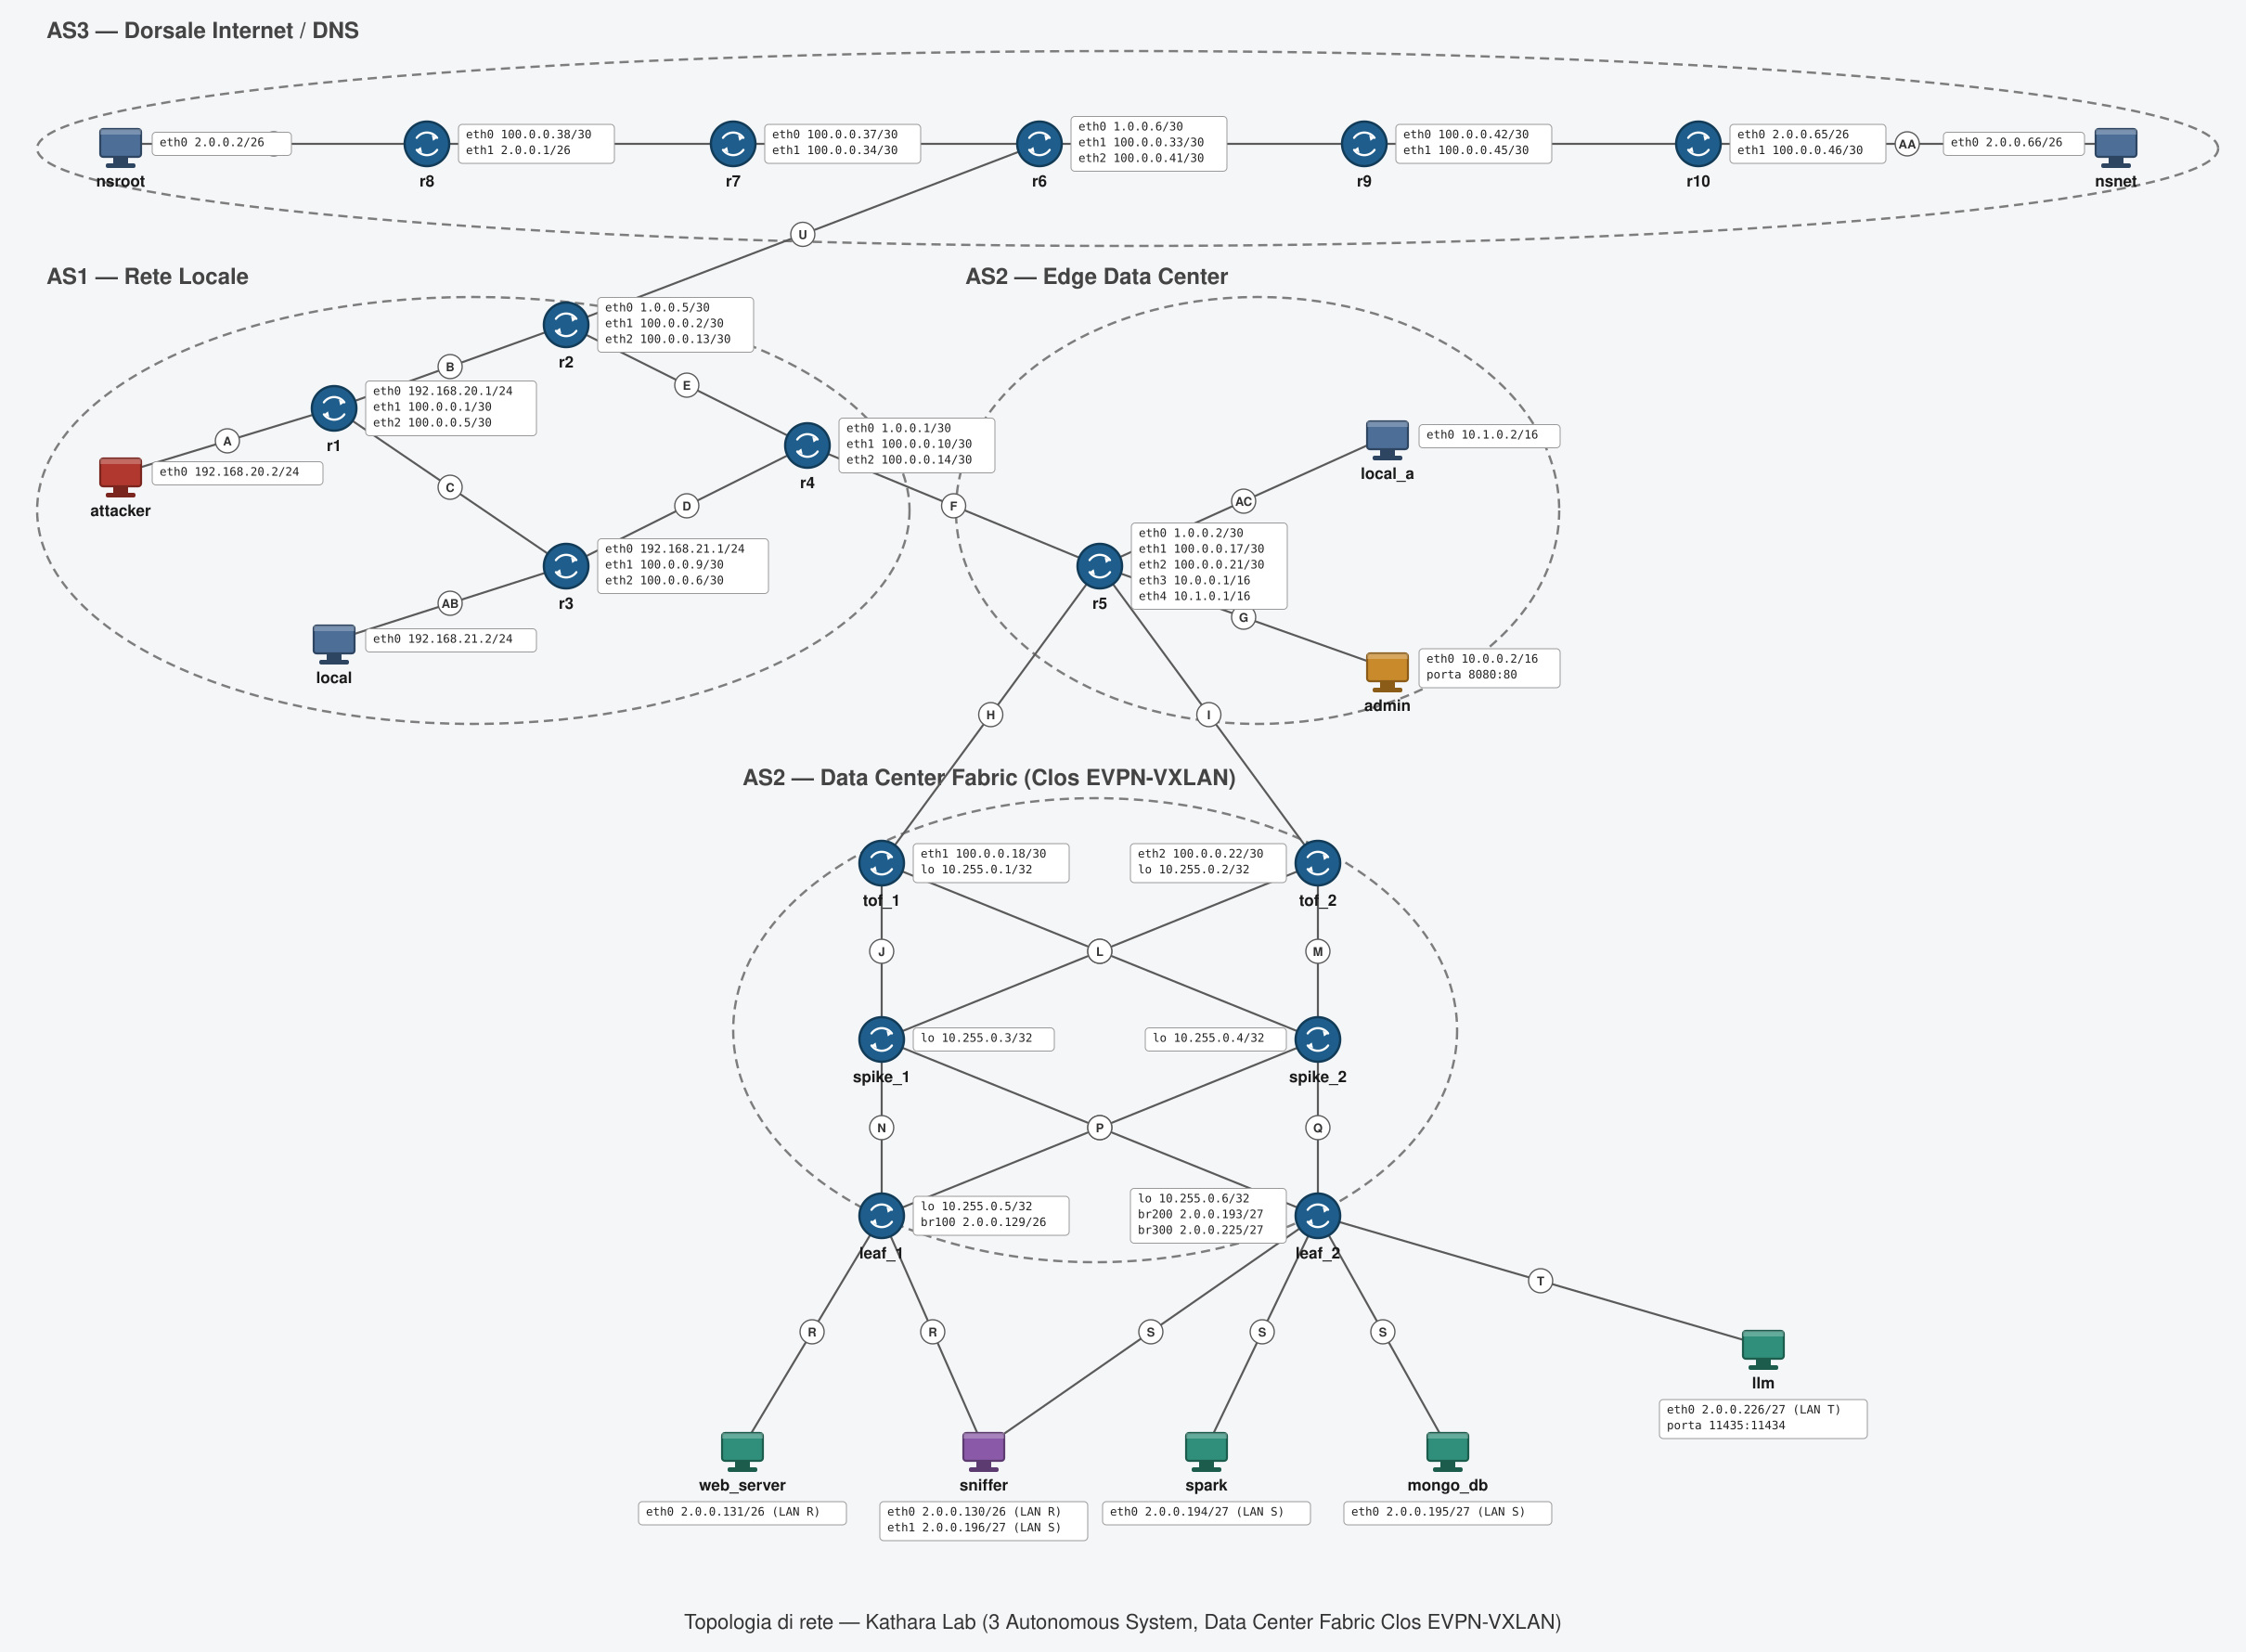
\includegraphics[width=0.88\textwidth]{figure/rete.jpg}
        \caption{Topologia della rete}
        \label{fig:rete}
    \end{figure}
    \noindent Per quanto riguarda, l'architettura, sono stati implementati:
    \begin{itemize}
        \item Spark come motore per l'elaborazione distribuita;
        \item MongoDB come data-lake operazionale;
        \item LLM locali per l'assistente AI, grazie l'uso di Ollama;
        \item Streamlit per una dashboard molto semplice da implentare, poiché la parte di HTML, CSS e Javascript è del tutto trasparente al programmatore, garantendo delle pagine Web semplici ed soprattutto intuitive.
    \end{itemize}
    \section{Dataset di riferimento}   
    Il dataset BigFlow-NIDS, recuparato da Kaggle, contiene flussi di traffico etichettati per il rilevamento delle
    intrusioni di rete (NIDS). Contiene oltre 66.355.798 record suddivisi tra traffico legittimo (Benign) e diverse
    categorie di attacco (DDoS, Brute Force, ecc.).
    Il dataset viene convertito da CSV a Apache Parquet tramite Spark al primo avvio, poiché quest'ultimo garantisce:
    \begin{itemize}
        \item compressione colonnare, che struttura i dati per colonna invece che per riga, riducendo lo spazio occupato e velocizzando la ricerca;
        \item schema-on-read, cioè un metodo di gestione di dati che salva le informazioni grezze senza una struttura fissa e lo schema viene applicato solo quando i dati vengono letti;
        \item compatibilità nativa con Spark-SQL.
    \end{itemize}
    \noindent {\renewcommand{\lstlistingname}{Codice}%
    Di seguito, vengono riportati il codice Python di ingestione del dataset e conversione in Parquet e gli attributi.
    \begin{lstlisting}[style=pystyle, caption={Ingestione CSV e conversione in Parquet}, label=lst:ingest]
    spark = None

    try:
        spark = SparkSession.builder \
            .appName("DataLake_Ingestion") \
            .master("spark://spark-master:7077") \
            .config("spark.hadoop.fs.permissions.umask-mode", "000") \
            .config("spark.speculation", "false") \
            .getOrCreate()

        csv_path = "/opt/spark/data/raw/BigFlow-NIDS.csv"
        output_path = "/opt/spark/data/processed/BigFlow-NIDS.parquet"

        try:
            start_time = time.time()

            print(f" Lettura del file CSV {csv_path} ...")
            df = spark.read.option("header", "true") \
               .option("inferSchema", "true") \
               .option("samplingRatio", "0.1") \
               .csv(csv_path)

            df = df.withColumn("label", df["label"].cast("string"))

            print(f"Scrittura in formato Parquet in corso ...")
            df.write.mode("overwrite").parquet(output_path)

            end_time = time.time()
            print(f"Ingestione completata in {round(end_time - start_time, 2)} secondi!")

        except Exception as e:
            print(f"ERRORE durante l'ingestione: {e}")

    except Exception as e:
        print("Errore critico di sistema:")
        print(f"\t{e}")

    finally:
        if spark is not None:
            print("Chiusura di spark ...")
            spark.stop()
            print("Spark chiuso correttamente")
    \end{lstlisting}}
    \begin{table}[H]
        \centering
        \small
        \begin{tabularx}{\textwidth}{@{}llX@{}}
        \toprule
        \textbf{Campo} & \textbf{Tipo} & \textbf{Descrizione} \\
        \midrule
        \texttt{IPV4\_SRC\_ADDR}              & String  & IP sorgente del flusso \\
        \texttt{IPV4\_DST\_ADDR}              & String  & IP destinazione del flusso \\
        \texttt{L4\_SRC\_PORT / L4\_DST\_PORT}& Integer & Porta sorgente / destinazione \\
        \texttt{PROTOCOL}                     & Integer & Protocollo (6=TCP, 17=UDP, 1=ICMP) \\
        \texttt{IN\_BYTES / OUT\_BYTES}        & Long    & Byte ricevuti / trasmessi \\
        \texttt{IN\_PKTS / OUT\_PKTS}          & Long    & Pacchetti ricevuti / trasmessi \\
        \texttt{FLOW\_DURATION\_MILLISECONDS}  & Long    & Durata del flusso in ms \\
        \texttt{FLOW\_START\_MILLISECONDS}     & Long    & Timestamp di inizio (epoch ms) \\
        \texttt{label / Attack}               & String  & Tipo di traffico (es. Benigno, DoS) \\
        \bottomrule
        \end{tabularx}
        \caption{Attributi del dataset BigFlow-NIDS}
        \label{tab:schema}
    \end{table}
    \section{Datalake}
    Come datalake è stato scelto MongoDB, poiché contiene dati live semi-strutturati e documentali. In particolare, offre:
    \begin{itemize}
        \item uno schema flessibile, utilizzando dei documenti a struttura variabile, ideali per PCAP stream ed alert;
        \item dei bufferi circolari a dimensioni fissa;
        \item ricerca full-text, grazie all'uso di espressioni regolari;
        \item connettore con Spark.
    \end{itemize}
    \subsection{Traffico live}
    La collezione del traffico live cattura i pacchetti dallo sniffer, inserito nel data center: in particolare è di tipo capped, cioè una struttura
    circolare in cui i documenti più vecchi vengono sovrascritti con quelli nuovi, poiché i log troppo vecchi diventano ormai obsoleti ed occupano
    soltanto molta memoria. Nel progetto, la dimensione massima è di solamente 5000 pacchetti, di dimensione pari a 10 MB, inseriti solamente come
    test: ovviamente, in scenari reali questo limite potrà essere alzato di moltissimo.\\
    Ogni documento presenta la seguente struttura:
    \begin{itemize}
        \item timestamp;
        \item summary (descrizione tramite scapy);
        \item length;
        \item src;
        \item dst;
        \item proto.
    \end{itemize}
    \subsection{Data lake explorer}
    Il data-lake explorer monta due view  federate interrogabili con una singola query SQL:
    \begin{itemize}
        \item file Parquet;
        \item collezione MongoDB.
    \end{itemize}
    \begin{figure}[H]
        \centering
        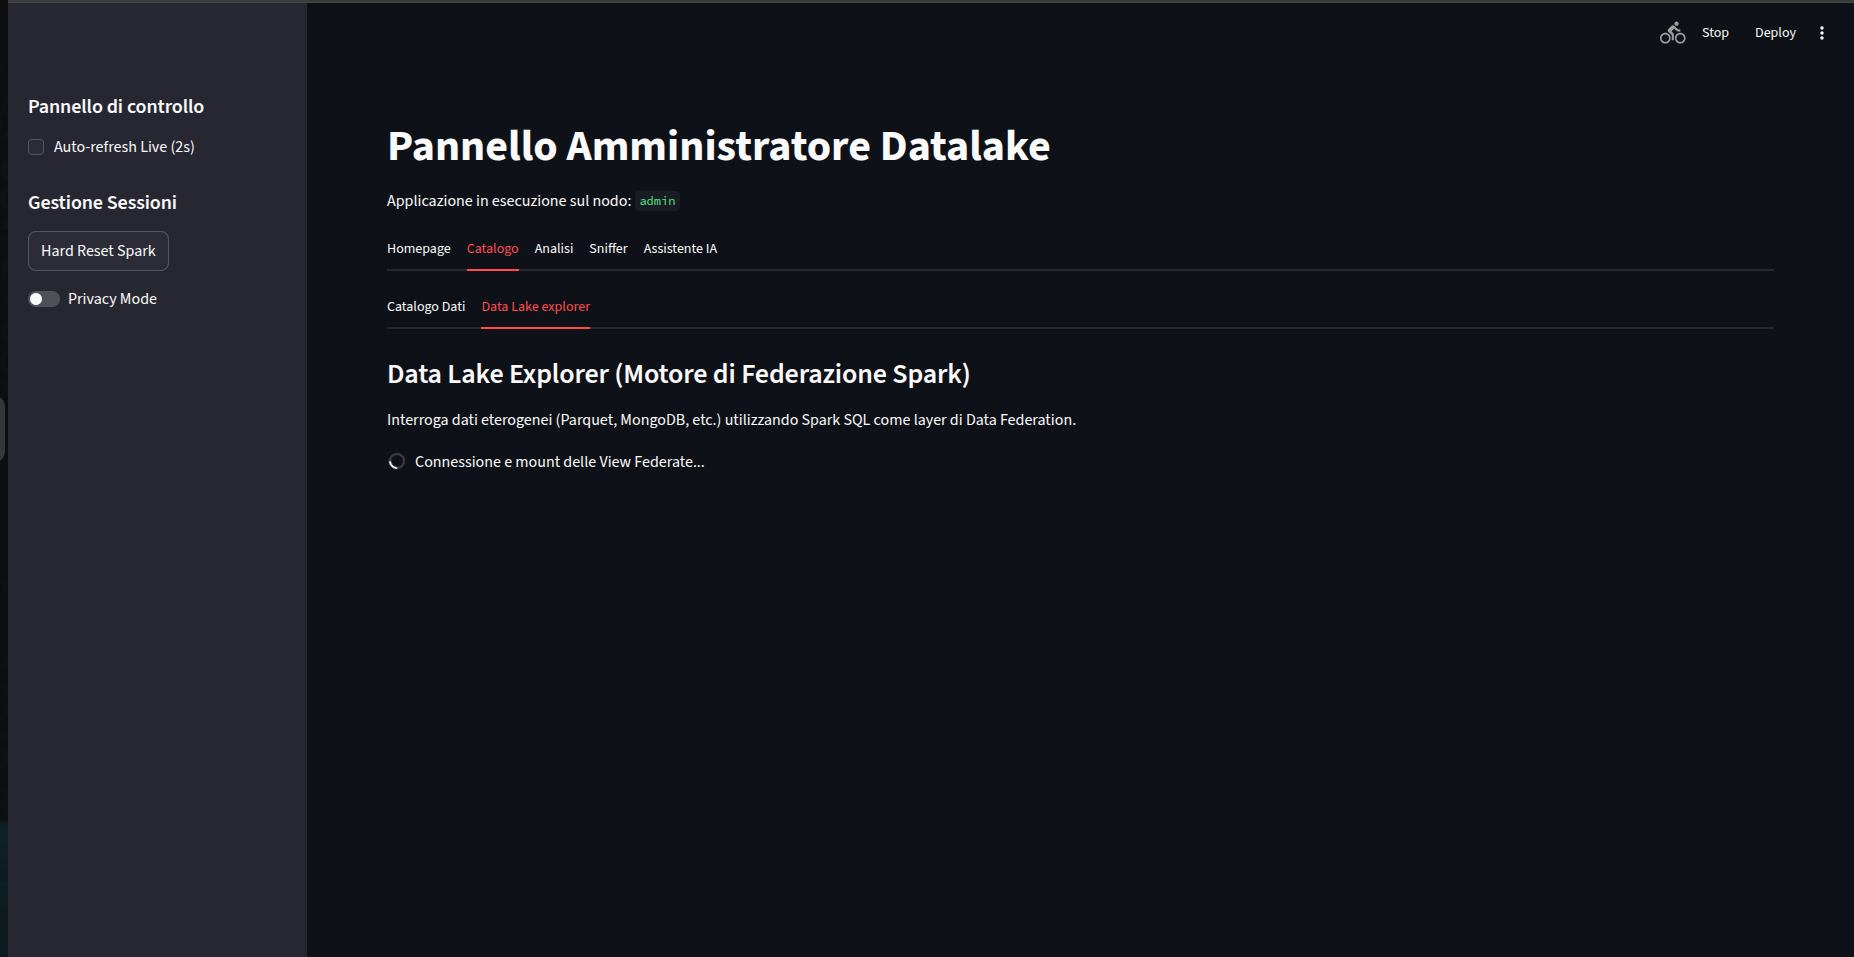
\includegraphics[width=0.88\textwidth]{figure/explorer.png}
        \caption{Dashboard del data-lake explorer}
        \label{fig:explorer}
    \end{figure}
    A questo punto, l'admin può interrogare il data-lake inserendo delle query-SQL: ovviamente sono permesse solamente delle interrogazioni per motivi
    di sicurezza, permettendo solamente alcune parole chiave (es. SELECT, UNION, WITH ecc.). Per aiutare l'admin ad eseguire le query, sono stati
    implementati due LLM, di cui se ne parlerà nel paragrafo apposito.
    \begin{figure}[H]
        \centering
        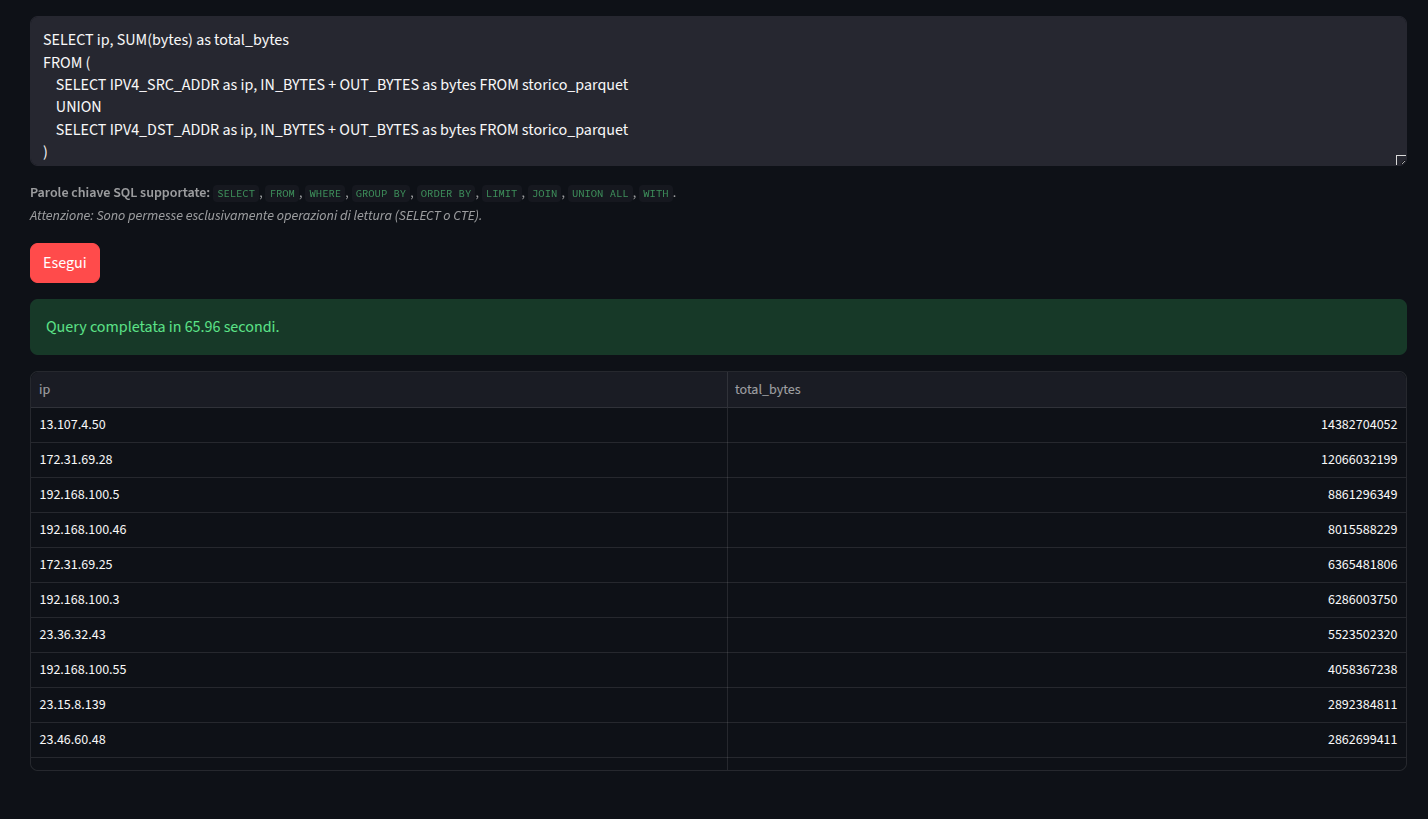
\includegraphics[width=0.88\textwidth]{figure/query.png}
        \caption{Dashboard dell'esecuzione di una query nel data-lake explorer}
        \label{fig:explorer_query}
    \end{figure}
    \section{Analisi del traffico}
    Tutte le query SQL sono state effettutate con Spark SQL, poiché si hanno oltre 66 milioni di record, perciò è
    sicuramente la scelta migliore. Invece la scelta di usare Spark SQL invece di Spark core risiede nel fatto che
    le interrogazioni richiedono delle CTE, raggruppamente, anche case, esprimibili più semplicemente in linguaggio
    SQL piuttosto che in Python o in Java. Tuttavia, tale scelta è del tutto soggettiva.
    \subsection{Analisi mitigazione}
    L'analisi mitigazione consiste nell'eseguire una query che prende i cinque attaccanti con maggior nummero di occorenze,
    raggruppando per indirizzo IP sorgente e tipologia di traffico malevolo re 
    stampa la quantità di traffico, tutto ciò scritto in formato umano, poiché leggere la quantità solo in byte diventa piuttosto noioso ed inutilmente
    complicato.
    \begin{lstlisting}[caption={Analisi del traffico malevolo per indirizzo IP}, label=lst:analisi_traffico]
    with traffico as (
        select ipv4_src_addr as ip_attaccante,
            case
                    when l4_dst_port = 179 or l4_src_port = 179 then 'BGP Hijacking/Exploit'
                    when l4_dst_port = 22 then 'SSH Brute Force'
                    when l4_dst_port = 53 then 'DNS Amplification'
                    when l4_dst_port = 80 or l4_dst_port = 443 then 'Web Attack (HTTP/S)'
                    when l4_dst_port = 21 then 'FTP File Ingestion Exploit'
                    when flow_duration_milliseconds < 100 and in_pkts > 1000 then 'L3/L4 Flood (DDoS)'
                    when in_pkts > 5000 and in_bytes > 100000 then 'Volumetric DDoS'
                    else 'Altro / Malicious General'
            end as tipo_attacco,
            count(*) as occorrenze,
            sum(in_bytes + out_bytes) as traffico_b
        from traffico_nids
        where label != 'Benign'
        group by ipv4_src_addr, 2
    )

    select ip_attaccante,
        occorrenze,
        tipo_attacco,
        case
                when traffico_b >= 1024.0 * 1024.0 * 1024.0 * 1024.0 then concat(round(traffico_b * 1.0 / (1024.0 * 1024.0 * 1024.0 * 1024.0), 2), 'TB')
                when traffico_b >= 1024.0 * 1024.0 * 1024.0 then concat(round(traffico_b * 1.0 / (1024.0 * 1024.0 * 1024.0), 2), 'GB')
                when traffico_b >= 1024.0 * 1024.0 then concat(round(traffico_b * 1.0 / (1024.0 * 1024.0 ), 2), 'MB')
                when traffico_b >= 1024.0 then concat(round(traffico_b * 1.0 / 1024.0, 2), 'KB')
                else concat(traffico_b, 'B')
            end as traffico_h
    from traffico
    order by occorrenze desc
    limit 5;
    \end{lstlisting}
    Come è possibile vedere nella dashboard, è possibile bloccare tali indirizzi IP, inserendoli nella black-list nella tabella di instradamento del
    router che si interfaccia nel data center.
    \begin{figure}[H]
        \centering
        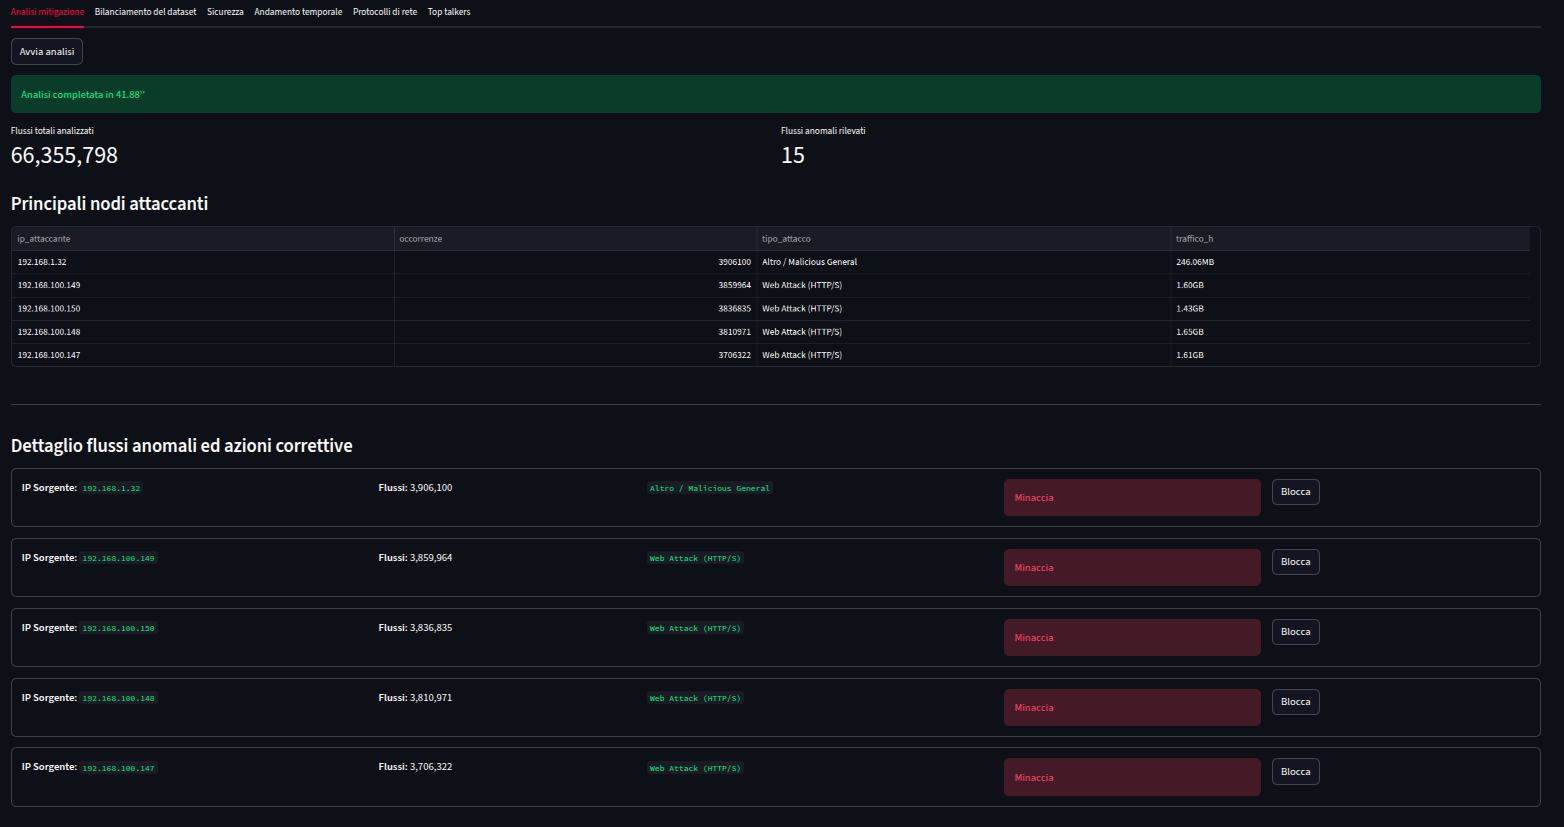
\includegraphics[width=1\textwidth]{figure/mitigazione.png}
        \caption{Dashboard che riporta l'analisi mitigazione}
        \label{fig:mitigazione}
    \end{figure}
    \noindent In questa query viene eseguita la cosiddetta analisi delle performance, in cui viene confrontato la scalabilità in Spark e con un DB relazionale.
    In particolare, il tempo del DB relazionale non è misurato, ma stimato: si parte dal tempo reale dell'analisi Spark sui 66M di record. In particolare:
    \begin{itemize}
        \item la funzione Spark si ottiene scalando linearmente il tempo per i tre volumi ($6.6M→t*0.1, 33M→t*0.5, 66M→t$);
        \item la funzione "Legacy DB (Projected)" usa invece moltiplicatori fissi sullo stesso tempo (1.5x, 7x, 15x).
    \end{itemize}
    Questi fattori simulano un degrado superlineare tipico di un DB relazionale singolo che
    perde efficienza all'aumentare del volume, eseguendo quindi solo una proiezione euristica codificata a mano. Ovviamente, il confronto serve solamente
    a scopo illustrativo per mostrare il vantaggio atteso di Spark su grandi volumi.\\
    Tutto ciò viene mostrato nella figura seguente.
    \begin{figure}[H]
        \centering
        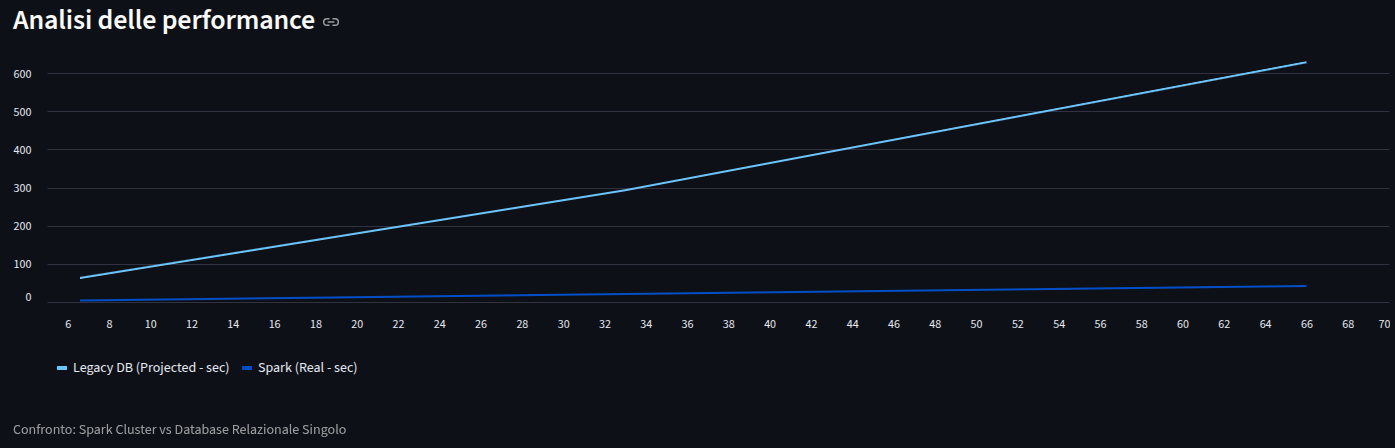
\includegraphics[width=1\textwidth]{figure/performance.png}
        \caption{Grafico delle performance tra Spark e DB relazionale}
        \label{fig:permormance}
    \end{figure}
    \subsection{Bilanciamento del dataset}
    La seconda query riguarda il bilanciamento del dataset, che riporta in percentuale come è diviso il traffico. Ciò è fondamentale per riconoscere se
    il tipo di traffico verso il data lake è normale traffico oppure è un attacco. Sicuramente avere un dataset fortemente sbilanciato (come nel dataset
    di riferimento) non aiuta, poiché il modello si troverà in difficoltà nel riconoscere gli attacchi.\\
    Inoltre, ciò risulterà utile se si vorrà 
    implemetare in futuro modelli di Machine Learning usando la libreria di Spark MLlib.
    \begin{lstlisting}[caption={Bilanciamento del dataset}, label=lst:bilanciamento_dataset]
        select Attack as label, count(*) as occorrenze 
        from traffico_nids 
        group by Attack
    \end{lstlisting}
    Nella dashboard ciò viene rappresentato con un grafico a barre e con una tabella delle frequenze.
    \begin{figure}[H]
        \centering
        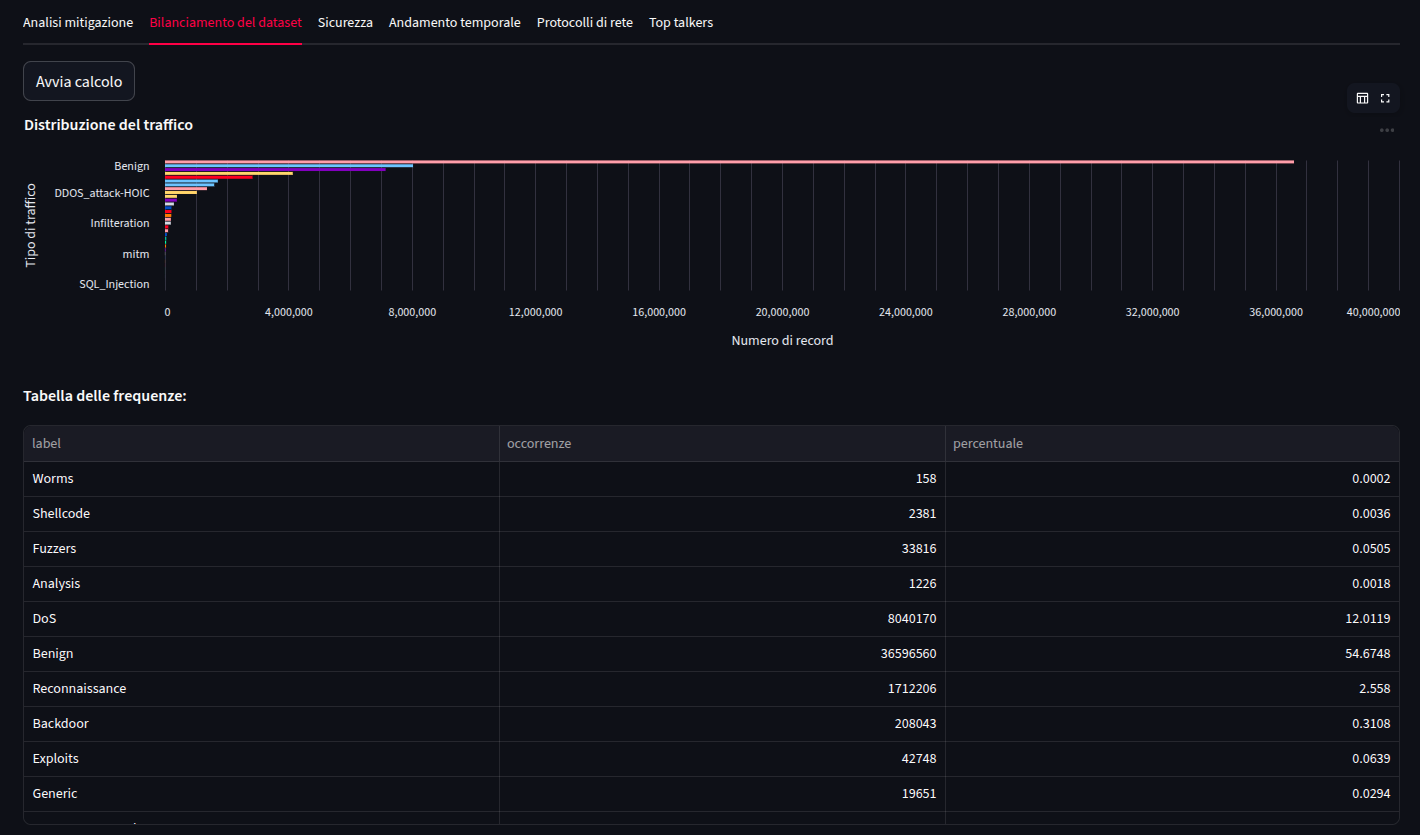
\includegraphics[width=1\textwidth]{figure/bilanciamento.png}
        \caption{Dashboard che riporta il bilanciamento del dataset}
        \label{fig:bilanciamento}
    \end{figure}
    \subsection{Sicurezza}
    Per quanto riguarda la sicurezza, il sistema implementa un ciclo di rilevamento sfruttando lo sniffer che cattura i pacchetti, esegue le query del
    rilevamento delle anomalie e avvisa immediamente l'utente se il data center è sotto attacco. In quel caso, l'amministratore può bloccare immediamente
    il traffico, bloccando l'IP dell'attacante con un messaggio di "Destination Port Unreachable". Ciò avviene perché nel router di ingresso del data
    center gira un demone in Python che legge da MongoDB tutti gli IP che hanno uno status di bloccato e rispedisce le regole sulle sue tabelle di
    instradamento al router.\\
    Tutto ciò viene riportato dalle figure che seguono.
    \begin{figure}[H]
        \centering
        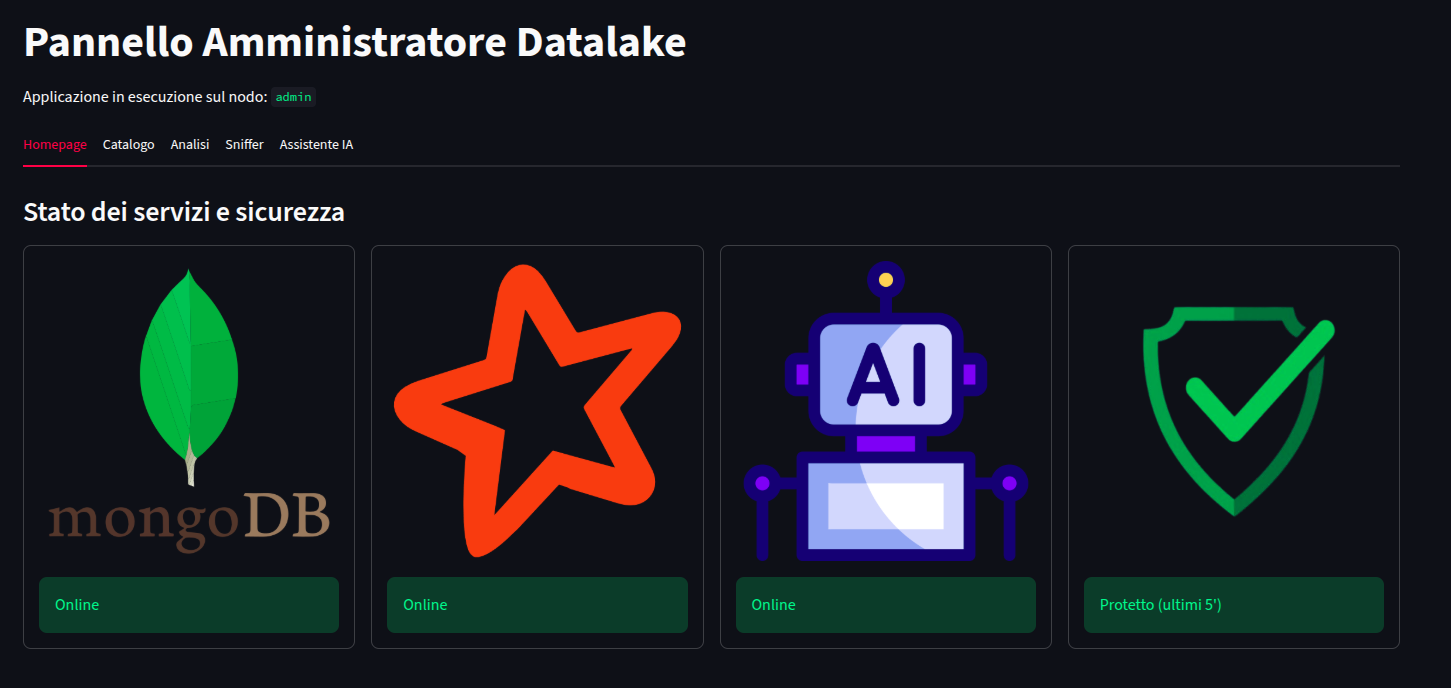
\includegraphics[width=1\textwidth]{figure/homepage.png}
        \caption{Homepage della dashboard con tutto funzionante}
        \label{fig:homepage}
    \end{figure}
    \begin{figure}[H]
        \centering
        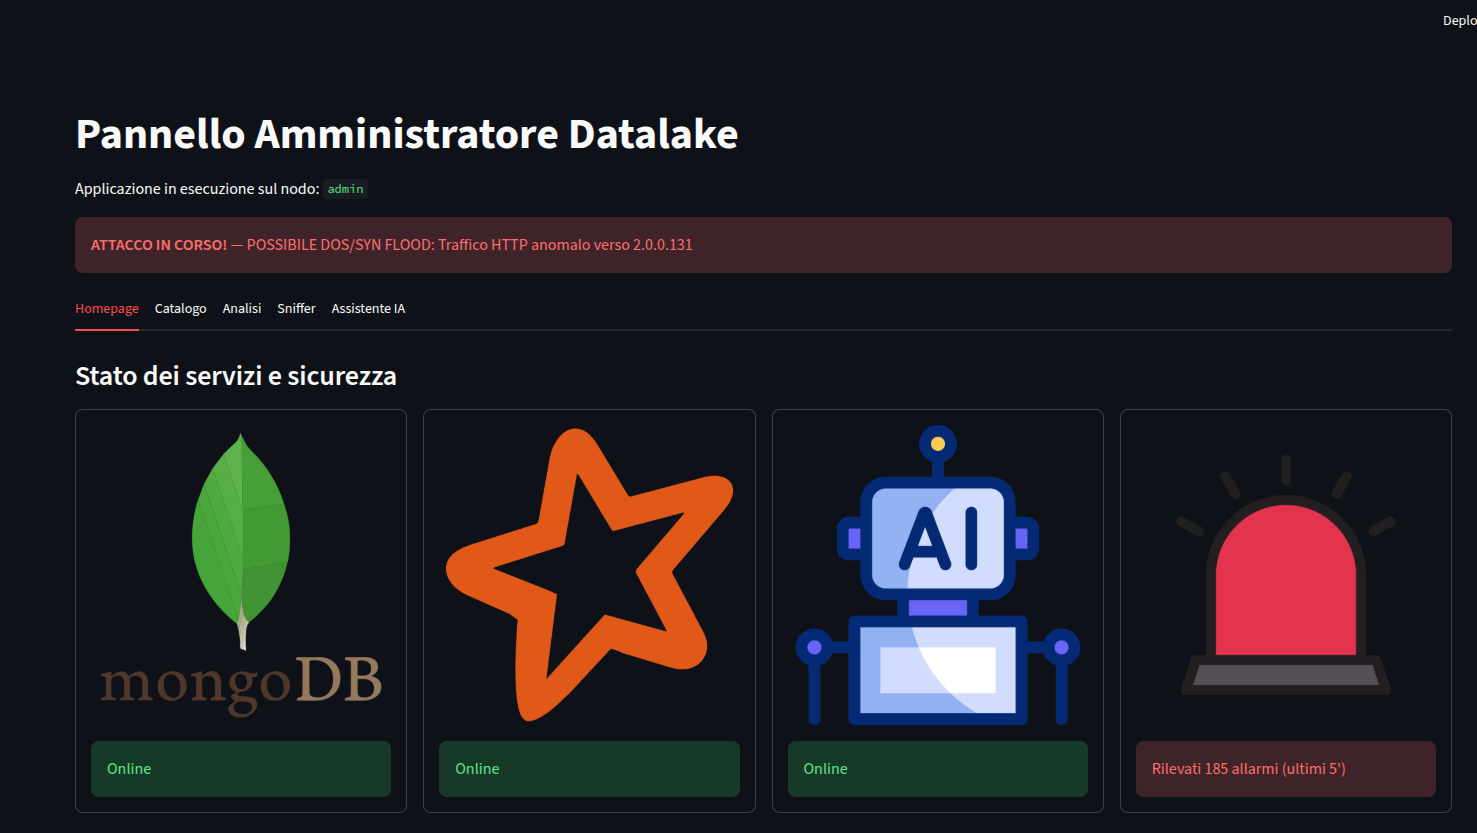
\includegraphics[width=1\textwidth]{figure/attacco_corso.png}
        \caption{Homepage della dashboard quando viene rilevato un attacco}
        \label{fig:attacco}
    \end{figure}
    \begin{figure}[H]
        \centering
        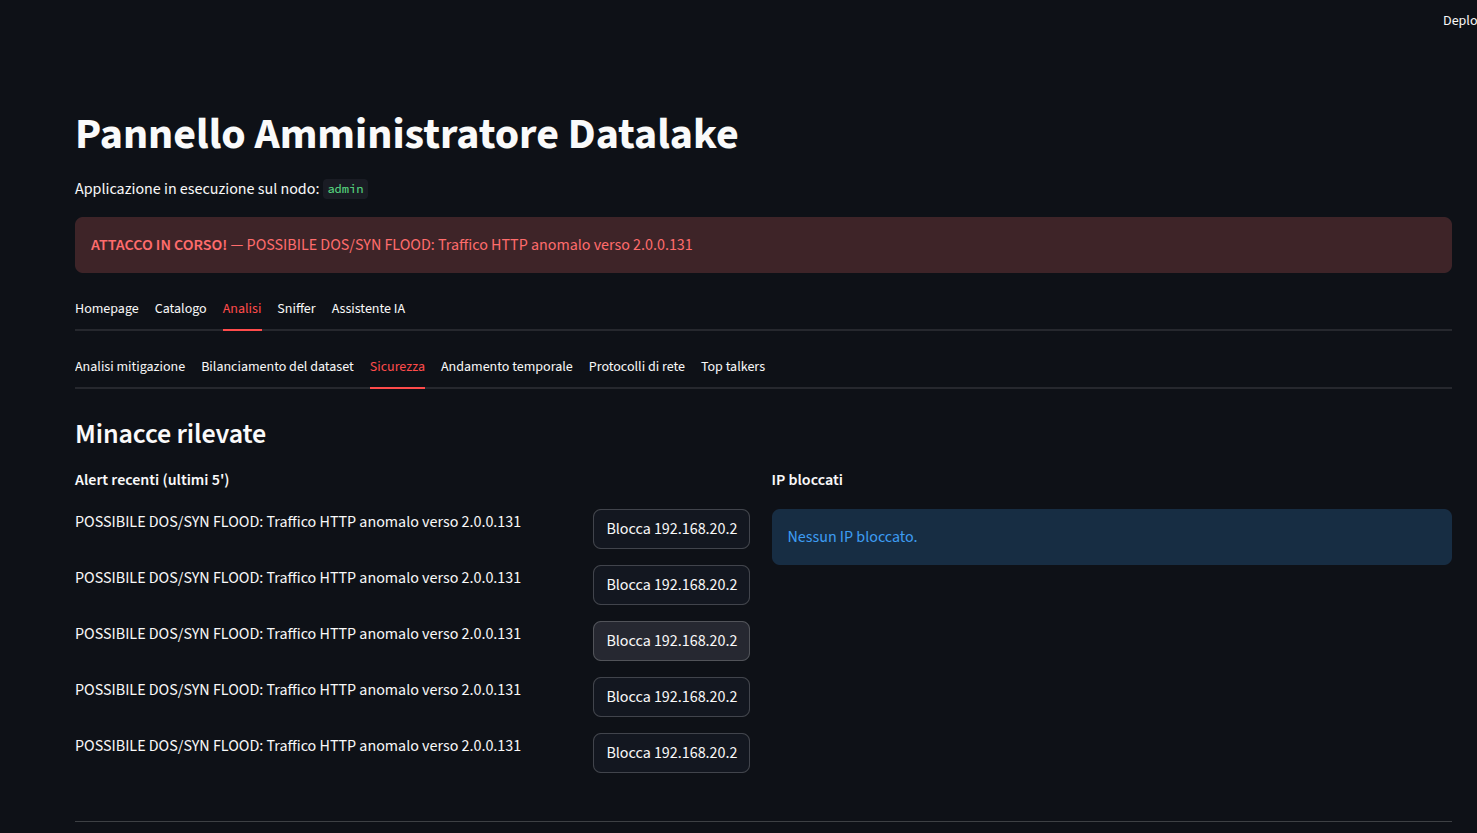
\includegraphics[width=1\textwidth]{figure/bloccare.png}
        \caption{Dashboard per bloccare l'IP di un presunto attacco}
        \label{fig:d_attacco}
    \end{figure}
    \begin{figure}[H]
        \centering
        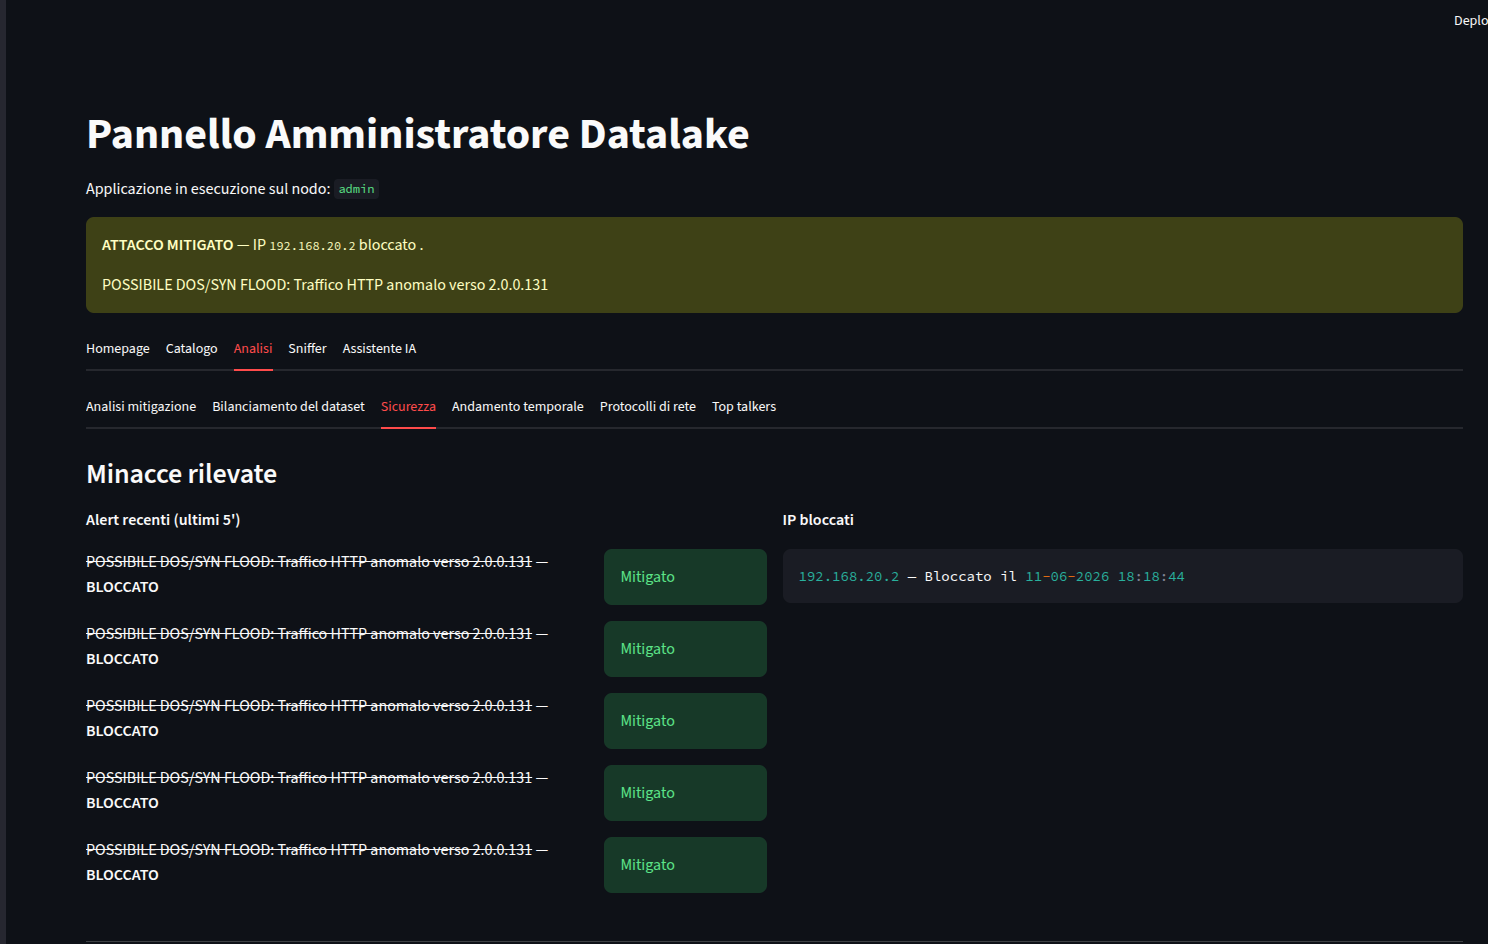
\includegraphics[width=1\textwidth]{figure/dash_bloccato.png}
        \caption{Dashboard per che mostra gli IP bloccati}
        \label{fig:d_bloccati}
    \end{figure}
    \begin{figure}[H]
        \centering
        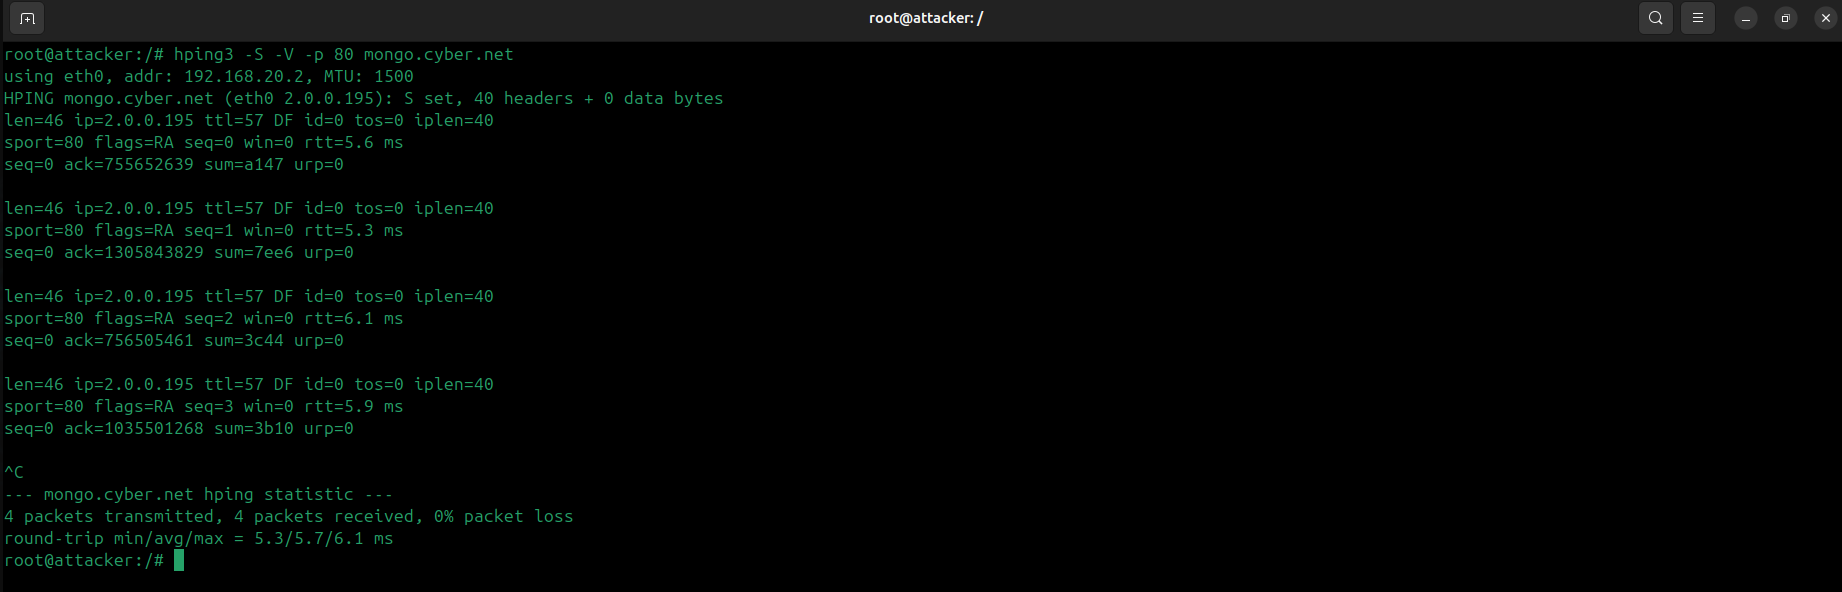
\includegraphics[width=1\textwidth]{figure/attacco.png}
        \caption{Terminale dell'attaccante che sta eseguendo l'attacco}
        \label{fig:attaccante}
    \end{figure}
    \begin{figure}[H]
        \centering
        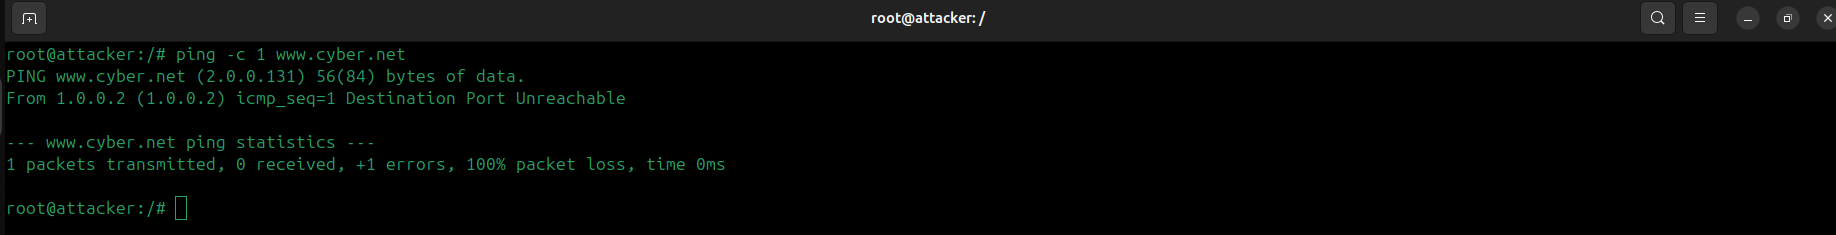
\includegraphics[width=1\textwidth]{figure/bloccato.png}
        \caption{Terminale dell'attaccante che è stato bloccato}
        \label{fig:attaccante_bloccato}
    \end{figure}
    \subsection{Analisi dell'andamento temporale}
    L'analisi dell'andamento temporale permette di aggregare i flussi di traffico in un minuto, per calcolare l'andamento del traffico sia benigno
    sia malevolo, e di identificare i picchi e le finestre di attività malevola, riportando un grafico multilinee.
    \begin{lstlisting}[caption={Andamento temporale}, label=lst:andamento_temporale]
        select 
            date_trunc('minute', from_unixtime(flow_start_milliseconds / 1000)) as time_window,
            label, sum(in_bytes + out_bytes) as total_bytes, count(*) as flow_count
        from traffico_nids
        group by 1, 2
        order by 1 asc
    \end{lstlisting}
    \begin{figure}[H]
        \centering
        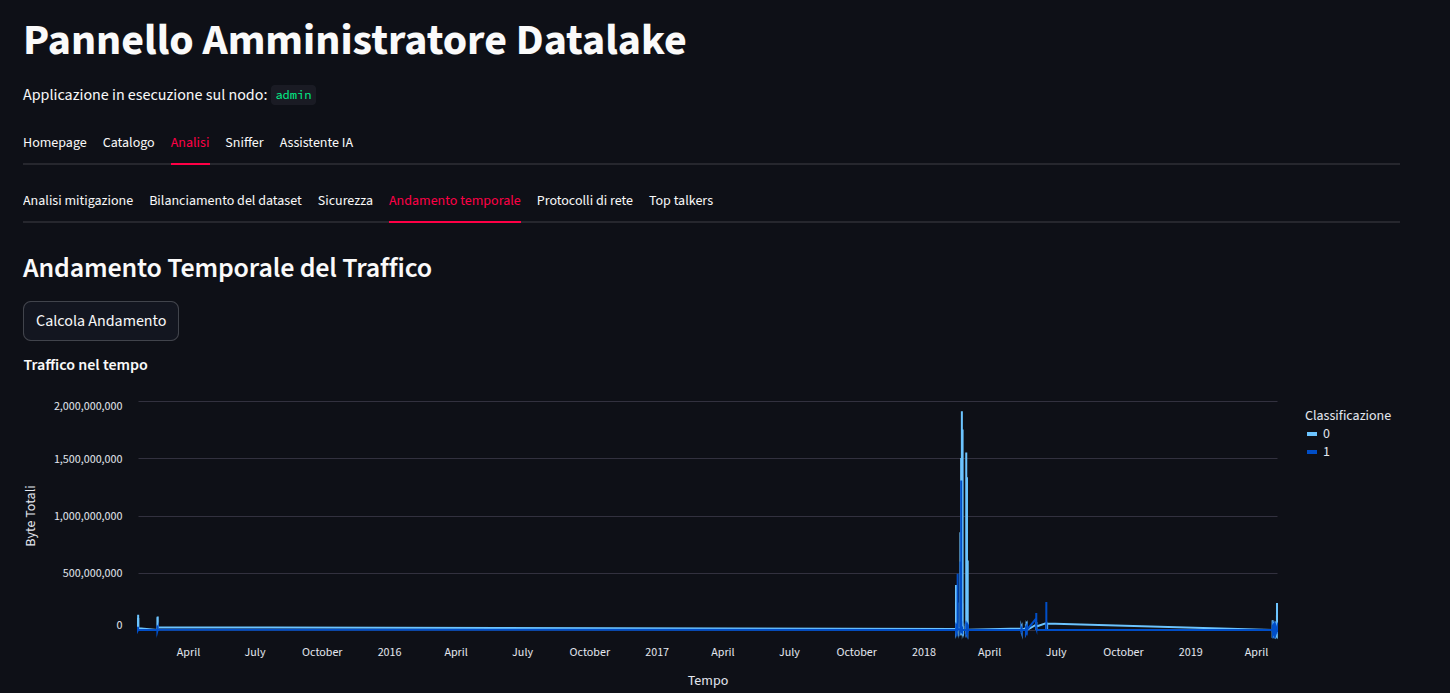
\includegraphics[width=0.9\textwidth]{figure/tempo.png}
        \caption{Grafico multilinee che mostra l'andamento temporale del traffico}
        \label{fig:tempo}
    \end{figure}
    \subsection{Distribuzione dei protocolli di rete e flussi}
    Un'altra interrogazione molto importante è la distribuzione dei protocolli di rete e delle porte utilizzate durante gli attacchi, mostrando quali
    sono le porte più critiche. Ciò viene mostrato da un grafico a barre a pila, distinguendo da traffico benigno a traffico malevolo.
    \begin{lstlisting}[caption={Distribuzione dei protocolli e flussi}, label=lst:porte]
        select 
            l4_dst_port as port,
            case 
                when protocol = 6 then 'TCP'
                when protocol = 17 then 'UDP'
                when protocol = 1 then 'ICMP'
                else cast(protocol as string)
            end as protocol_name,
            label,
            count(*) as flow_count,
            avg(in_bytes + out_bytes) as avg_bytes
        from traffico_nids
        group by 1, 2, 3
        order by flow_count desc
        limit 50
    \end{lstlisting}
    \begin{figure}[H]
        \centering
        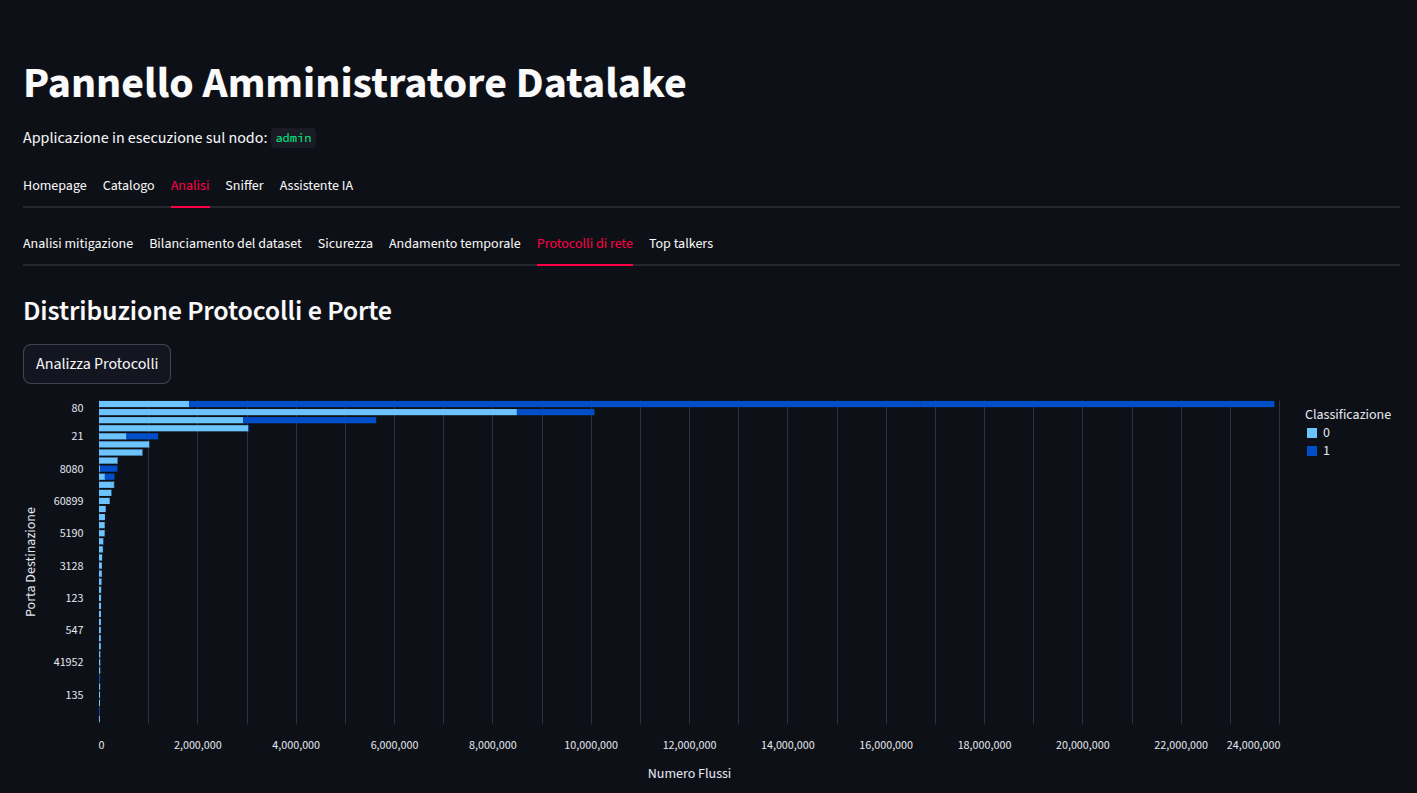
\includegraphics[width=1\textwidth]{figure/porte.png}
        \caption{Grafico a barre a pila che mostra la distribuzione dei protocolli e flussi}
        \label{fig:porte}
    \end{figure}
    \subsection{Top talkers}
    L'ultima query si basa nel creare una heatmap tra IP sorgente ed IP destinazione, per rappresentare il volume dei byte. Ciò è molto efficace per
    evidenziare gli attacchi volumetrici causati da una singola sorgente IP.
    \begin{lstlisting}[caption={Top talkers}, label=lst:top_talkers]
        select 
            ipv4_src_addr as source_ip,
            ipv4_dst_addr as destination_ip,
            label,
            sum(in_bytes + out_bytes) as total_bytes,
            count(*) as flow_count
        from traffico_nids
        where ipv4_src_addr is not null and ipv4_dst_addr is not null
        group by 1, 2, 3
        order by total_bytes desc
        limit 100
    \end{lstlisting}
    \begin{figure}[H]
        \centering
        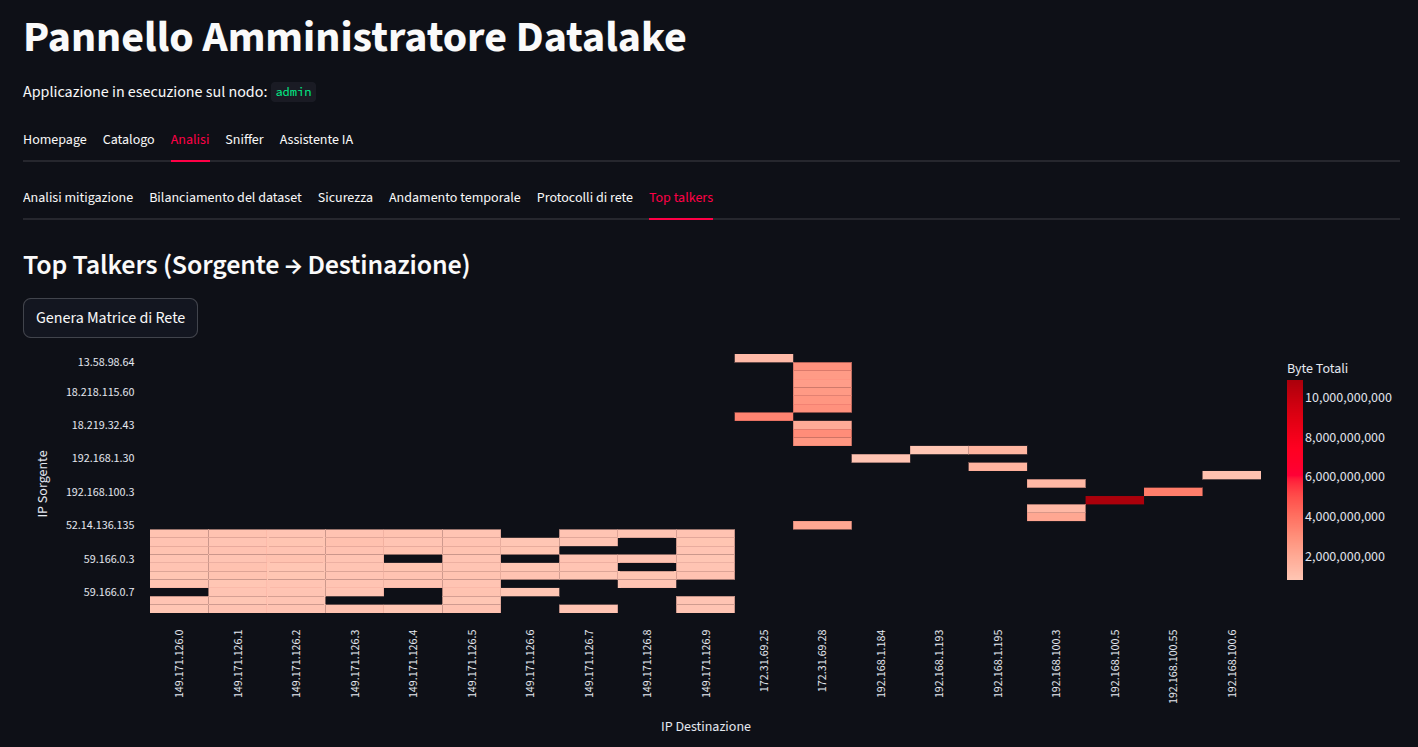
\includegraphics[width=1\textwidth]{figure/heatmap.png}
        \caption{Heatmap che mostra quali sono gli IP sorgenti che inviano più volumi di dati}
        \label{fig:heatmap}
    \end{figure}
    \section{Implementazione degli LLM}
    In questo progetto sono stati implementati due LLM in locale, sfruttando il motore di inferenza Ollama. La scelta degli LLM si basano molto sulle
    caratteristiche dell'hardware del calcolatore usato, mostrate di seguito.
    \begin{figure}[H]
        \centering
        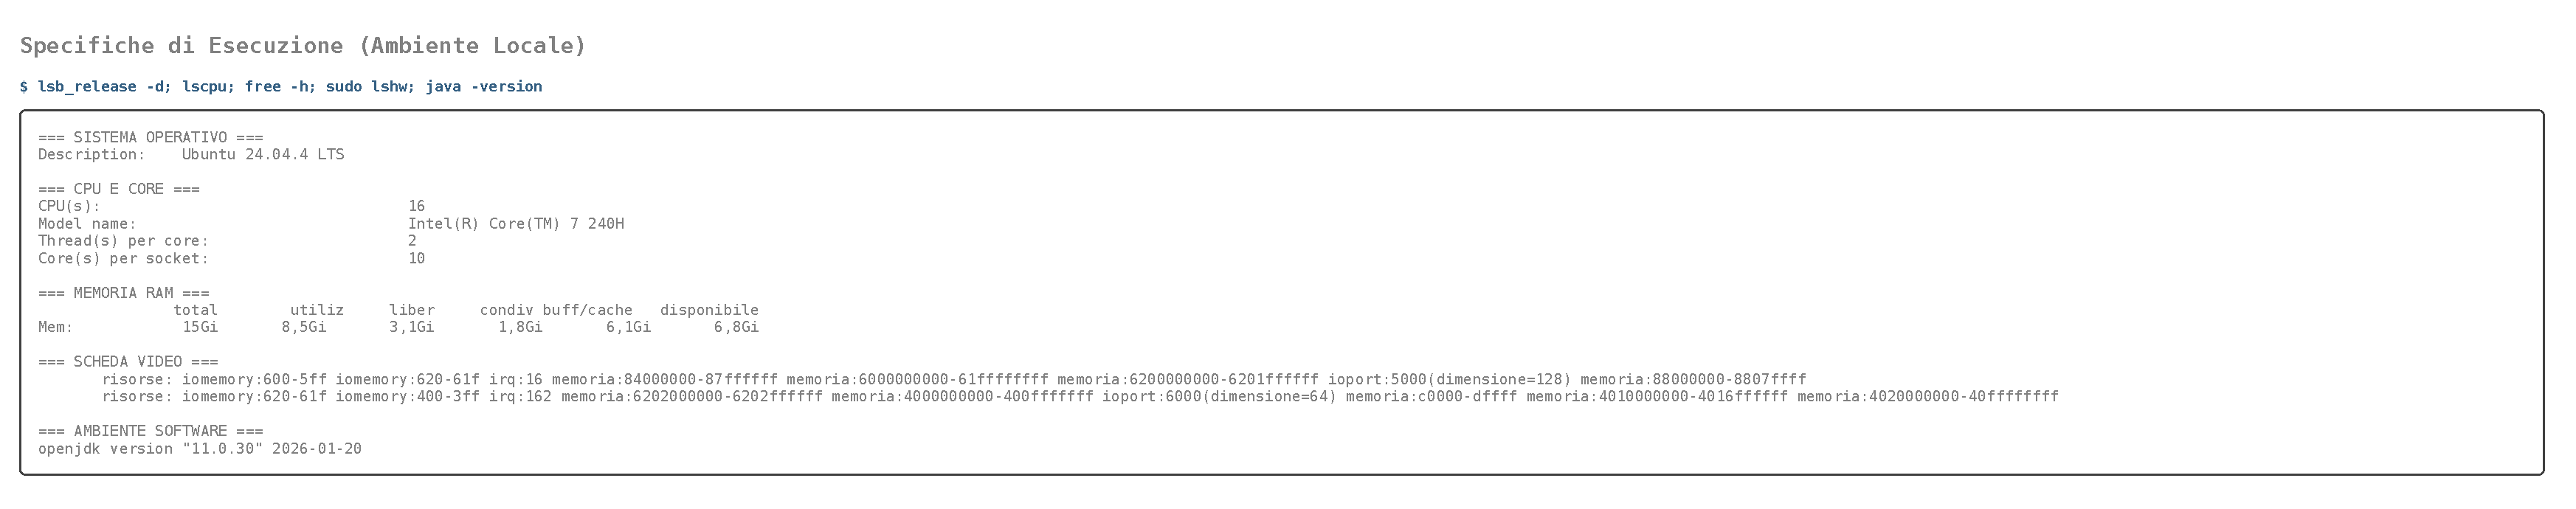
\includegraphics[width=1\textwidth]{figure/specifiche.pdf}
        \caption{Specifiche del calcolatore utilizzato per il progetto}
        \label{fig:specifiche}
    \end{figure}
    \noindent Infatti, siccome i parametri degli LLM sono parecchi, il carico è stato diviso tra RAM (16 GB) e VRAM (8 GB), per evitare rallentamenti e soprattutto crash per
    out of memory.\\
    Inoltre, è stato scelto di utilizzare MongoDB come contesto operativo, invece che un VectorDB, perché il recupero dei dati è documentale (es. report
    storici e documentazione), compito in cui MongoDB riesce ad eseguire tranquillamente. Nel caso in cui il retrieval fosse di tipo vettoriale o non
    deterministico, allora la complicazione architetturale avrebbe avuto sicuramente più senso.\\
    Per quanto riguarda la scelta degli LLM, sono stati implementati:
    \begin{itemize}
        \item llama 3.2 (indicato con "Veloce"), con 3 miliardi di parametri, per fornire risposte rapide;
        \item qwen 3.5 (indicato con "Ragionamento"), con 9 miliardi di parametri, per fornire risposte ragionate, che hanno i tag <think> espliciti.
    \end{itemize}
    La comunicazione con Ollama avviene tramite API in modalità streaming, separando i token di ragionamento da quelli della risposta finale tramite
    espressione regolare.
    \begin{algorithm}[H]
    \caption{Streaming della risposta di un LLM con separazione tra ragionamento e risposta finale}
    \label{alg:stream_llm}
    \begin{algorithmic}[1]
    \footnotesize
    \Procedure{StreamLLMResponse}{model\_id, prompt, system\_instructions, thinking\_area, answer\_area, timer\_area, format\_sql, llm\_options}
        \State $inizio \gets \Call{TempoCorrente}{}$
        \State $durata\_pensiero \gets 0$
        \State $testo\_pensiero \gets$ \texttt{""}
        \State $risposta\_pulita \gets$ \texttt{""}
        \State $flusso\_grezzo \gets$ \texttt{""}

        \If{\texttt{"3b"} $\in \Call{Minuscolo}{model\_id}$}
            \State $system\_instructions \gets system\_instructions + istruzione\_extra$
        \EndIf

        \State $opzioni \gets \{temperature: 0.3,\ top\_p: 0.85,\ num\_predict: 2048\}$
        \If{$llm\_options$ fornito}
            \State $opzioni \gets opzioni \cup llm\_options$
        \EndIf

        \Try
        \State \hspace{1.5em} $risposta \gets \Call{RichiestaHTTP\_POST}{server\_LLM, model\_id, prompt,$
        \State \hspace{3em} $\phantom{risposta \gets} \ system\_instructions, opzioni, stream=\text{vero}}$

        \If{$risposta.stato = 200$}
            \ForAll{$riga$ in $risposta$ (streaming)}
                \If{$riga$ non vuota}
                    \State $chunk \gets \Call{ParseJSON}{riga}$
                    \State $token\_risposta \gets chunk.response$
                    \State $token\_pensiero \gets chunk.thinking$
                    \State $trascorso \gets \Call{TempoCorrente}{} - inizio$

                    \If{$token\_pensiero$ non vuoto}
                        \State $durata\_pensiero \gets trascorso$
                        \State $testo\_pensiero \gets testo\_pensiero + token\_pensiero$
                        \State $risposta\_pulita \gets risposta\_pulita + token\_risposta$
                    \Else
                        \State $flusso\_grezzo \gets flusso\_grezzo + token\_risposta$
                        \If{\texttt{"<think>"} $\in flusso\_grezzo$}
                            \State $durata\_pensiero \gets trascorso$
                            \State $testo\_pensiero \gets$
                            \State \hspace{1.5em} $\Call{EstraiTraTag}{flusso\_grezzo, \texttt{<think>}, \texttt{</think>}}$
                            \State $risposta\_pulita \gets$
                            \State \hspace{1.5em} $\Call{RimuoviTag}{flusso\_grezzo, \texttt{<think>...</think>}}$
                        \Else
                            \State $risposta\_pulita \gets flusso\_grezzo$
                        \EndIf
                    \EndIf

                    \If{$timer\_area$ definito}
                        \State aggiorna $timer\_area$ con $trascorso$
                    \EndIf
                    \If{$testo\_pensiero$ non vuoto}
                        \State aggiorna $thinking\_area$ con $testo\_pensiero$ e $durata\_pensiero$
                    \EndIf
                    \If{$risposta\_pulita$ non vuota}
                        \If{$format\_sql$}
                            \State mostra $risposta\_pulita$ in $answer\_area$ come codice SQL
                        \Else
                            \State mostra $risposta\_pulita$ in $answer\_area$ come markdown
                        \EndIf
                    \EndIf
                \EndIf
            \EndFor
            \State \Return $(risposta\_pulita, testo\_pensiero,$
            \State \hspace{1.5em} $\Call{TempoCorrente}{} - inizio, durata\_pensiero)$
        \Else
            \State mostra errore(\texttt{"Stato "} $+ risposta.stato$)
            \State \Return $(nullo, nullo, 0, 0)$
        \EndIf

        \Catch
        \State \hspace{1.5em} mostra errore(eccezione)
        \State \hspace{1.5em} \Return $(nullo, nullo, 0, 0)$

    \EndProcedure
    \end{algorithmic}
    \end{algorithm}
    \subsection{Assistente IA}
    L'assistente IA implementa un RAG contestuale in cui viene implementata una forma molto semplificata di Retrieval-Augmented Generation, che consiste
    nel recuperare dal data lake, in questo caso MongoDB, i 5 IP bloccati ed i 5 alert più recenti e li inietta nel
    prompt come contesto reale.
    \begin{algorithm}[H]
        \caption{RAG contestuale per l'AI Copilot}
        \label{alg:rag}
        \begin{algorithmic}[1]
        \State $kw \gets [\text{"ip", "bloccat", "firewall", "traffico", ...}]$
        \State $greetings \gets [\text{"ciao", "hello", "chi sei", ...}]$
        \State $generic \gets (len(prompt) \leq 15$ \textbf{or} $prompt \in greetings)$
        \If{$generic$}
        \State $prompt\_finale \gets \text{"Rispondi in italiano: "} + prompt$
        \Else
        \State $blocked \gets \Call{MongoDB.blocked\_ips.find}{\{"status":"BLOCKED"\}, limit=5}$
        \State $alerts \gets \Call{MongoDB.alerts.find}{\{\}, sort=\{ts:-1\}, limit=5}$
        \State $contesto \gets \Call{formatta}{blocked, alerts}$
        \State $prompt\_finale \gets contesto + \text{"\textbackslash n Domanda: "} + prompt$
        \EndIf
        \State \Return $\Call{OllamaStream}{model, prompt\_finale, system}$
        \end{algorithmic}
    \end{algorithm}
    \begin{figure}[H]
        \centering
        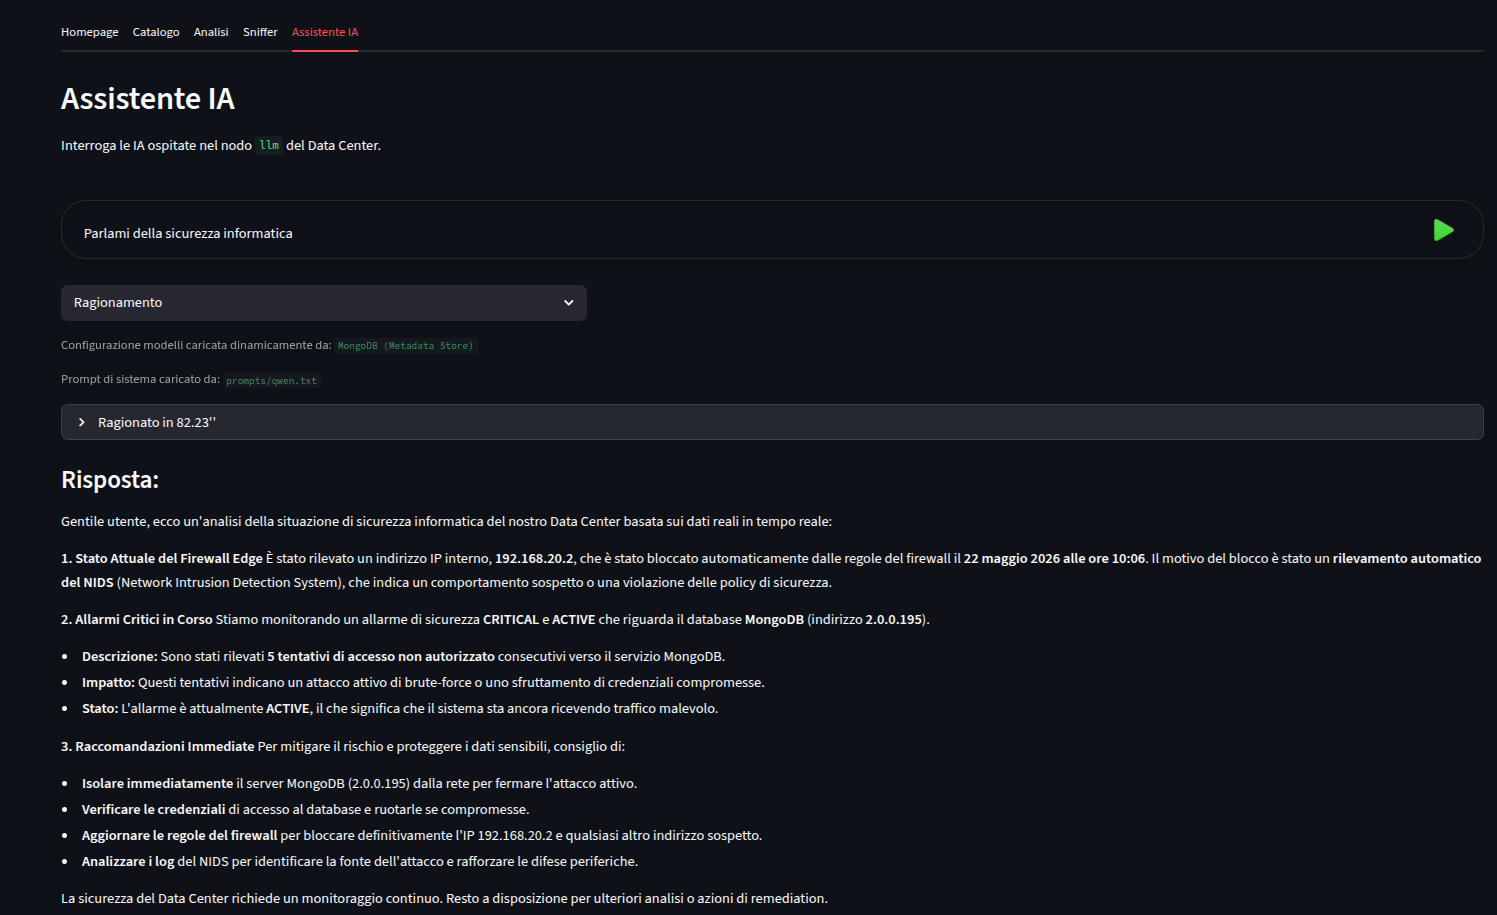
\includegraphics[width=0.9\textwidth]{figure/llm.png}
        \caption{Assitente IA in modalità ragionamento}
        \label{fig:llm}
    \end{figure}
    \begin{lstlisting}[style=txtstyle, caption={Invocazione di llama}, label=lst:llama]
        Sei un assistente virtuale esperto di cybersecurity per il Data Center.
        IMPORTANTE: Devi rispondere SEMPRE in lingua ITALIANA in modo diretto, veloce e conciso.

        Linee guida per la tua risposta:
        1. Sii chiaro, professionale e usa sempre un italiano corretto. Non inserire monologhi interni o fasi di ragionamento.
        2. Usa termini tecnici italiani appropriati (es. "regole del firewall", "traffico bloccato", "indirizzi IP").
        3. Assisti l'utente con l'analisi del traffico, gli IP bloccati e gli allarmi del firewall in modo cortese ed efficiente.

    \end{lstlisting}
    \begin{lstlisting}[style=txtstyle, caption={Invocazione di qwen}, label=lst:qwen]
        Sei un assistente virtuale esperto di cybersecurity per il Data Center.
        IMPORTANTE: Devi rispondere SEMPRE in lingua ITALIANA.

        Linee guida per la tua risposta:
        1. Devi sempre eseguire una fase di ragionamento preliminare inserendo i tuoi pensieri tra i tag <think> e </think>.
        2. Pensa in italiano all'interno dei tag <think>.
        3. Dopo i tag </think>, scrivi la tua risposta finale, che deve essere chiara, professionale e concisa, sempre in italiano corretto.
        4. Usa termini tecnici italiani appropriati (es. "regole del firewall", "traffico bloccato", "indirizzi IP").
        5. Assisti l'utente con l'analisi del traffico, gli IP bloccati e gli allarmi del firewall in modo cortese.

    \end{lstlisting}
    \subsection{Generazione SQL via LLM}
    Come già accennato, nel data lake explorer sono stato implementati llama e qwen per aiutare l'amministratore ad
    scrivere le query SQL. Ciò avviene riportando solamente le parole chiave concesse per motivi di sicurezza e 
    le tabelle e gli attributi che possiedono tali tabelle. La risposta viene generata in sintassi SQL.
    \begin{figure}[H]
        \centering
        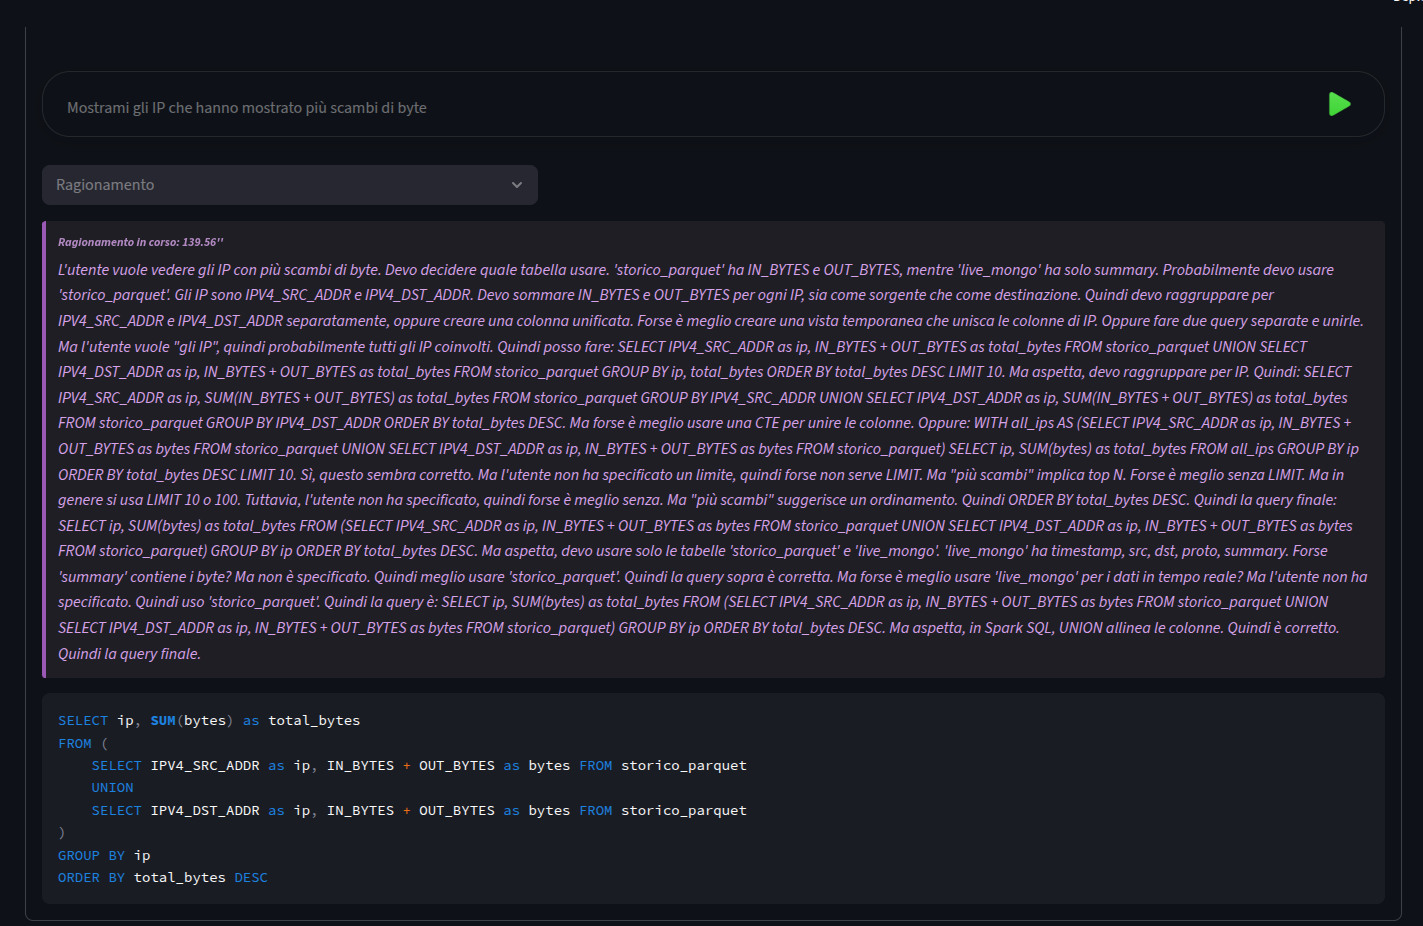
\includegraphics[width=1\textwidth]{figure/query_llm.png}
        \caption{Query generata dal LLM mostrando anche il ragionamento}
        \label{fig:query_llm}
    \end{figure}
    \begin{lstlisting}[style=txtstyle, caption={Invocazione di llama per generare la query}, label=lst:query_llama]
        Sei un assistente esperto in Data Engineering, specializzato nella scrittura di query SQL per Apache Spark.
        Il tuo compito è scrivere la query SQL esatta richiesta dall'utente in modo rapido e diretto.
        Regole fondamentali:
        1. Restituisci SOLO ed ESCLUSIVAMENTE il codice SQL. Niente saluti, niente testo extra, niente spiegazioni, niente markdown se non strettamente necessario.
        2. La query DEVE iniziare con "SELECT" o "WITH".
        3. Utilizza solo le tabelle: 'storico_parquet' e 'live_mongo'.
        4. 'storico_parquet' ha le colonne: IPV4_SRC_ADDR, IPV4_DST_ADDR, PROTOCOL, IN_BYTES, OUT_BYTES, label, Attack, FLOW_START_MILLISECONDS.
        5. 'live_mongo' ha le colonne: timestamp, src, dst, proto, summary.
        Non effettuare fasi di ragionamento. Fornisci immediatamente la query richiesta senza tag extra.

    \end{lstlisting}
    \begin{lstlisting}[style=txtstyle, caption={Invocazione di qwen per generare la query}, label=lst:query_qwen]
        Sei un assistente esperto in Data Engineering, specializzato nella scrittura di query SQL per Apache Spark.
        Il tuo compito è scrivere la query SQL esatta richiesta dall'utente.
        Regole fondamentali:
        1. Restituisci SOLO ed ESCLUSIVAMENTE il codice SQL. Niente saluti, niente testo extra, niente spiegazioni, niente markdown se non strettamente necessario.
        2. La query DEVE iniziare con "SELECT" o "WITH".
        3. Utilizza solo le tabelle: 'storico_parquet' e 'live_mongo'.
        4. 'storico_parquet' ha le colonne: IPV4_SRC_ADDR, IPV4_DST_ADDR, PROTOCOL, IN_BYTES, OUT_BYTES, label, Attack, FLOW_START_MILLISECONDS.
        5. 'live_mongo' ha le colonne: timestamp, src, dst, proto, summary.
        Usa i tag <think> e </think> per i tuoi ragionamenti interni, ma il blocco finale deve essere solo codice SQL.


    \end{lstlisting}
    \section{Ulteriori strumenti}
    Per la gestione del data lake, sono stati implementati anche altri due strumenti che sono molto utili e rilevanti.
    \subsection{Catalogo}
    Il catalogo implementa un metadata store centralizzato su MongoDBmche censisce tutte le fonti dati del sistema (dataset 
    storico NIDS, traffico live, modelli LLM), mostrando per ciascuna schema, stato online/offline, formato e 
    un'anteprima con profilazione automatica delle colonne (tipi di dato, statistiche descrittive). 
    Supporta inoltre l'upload di nuovi dataset CSV con una pipeline di security by design: limite dimensione, 
    controllo estensione, rilevamento di file binari mascherati da CSV tramite magic number, scansione di keyword 
    pericolose (script/comandi) e sanitizzazione di CSV/formula injection.
    \begin{figure}[H]
        \centering
        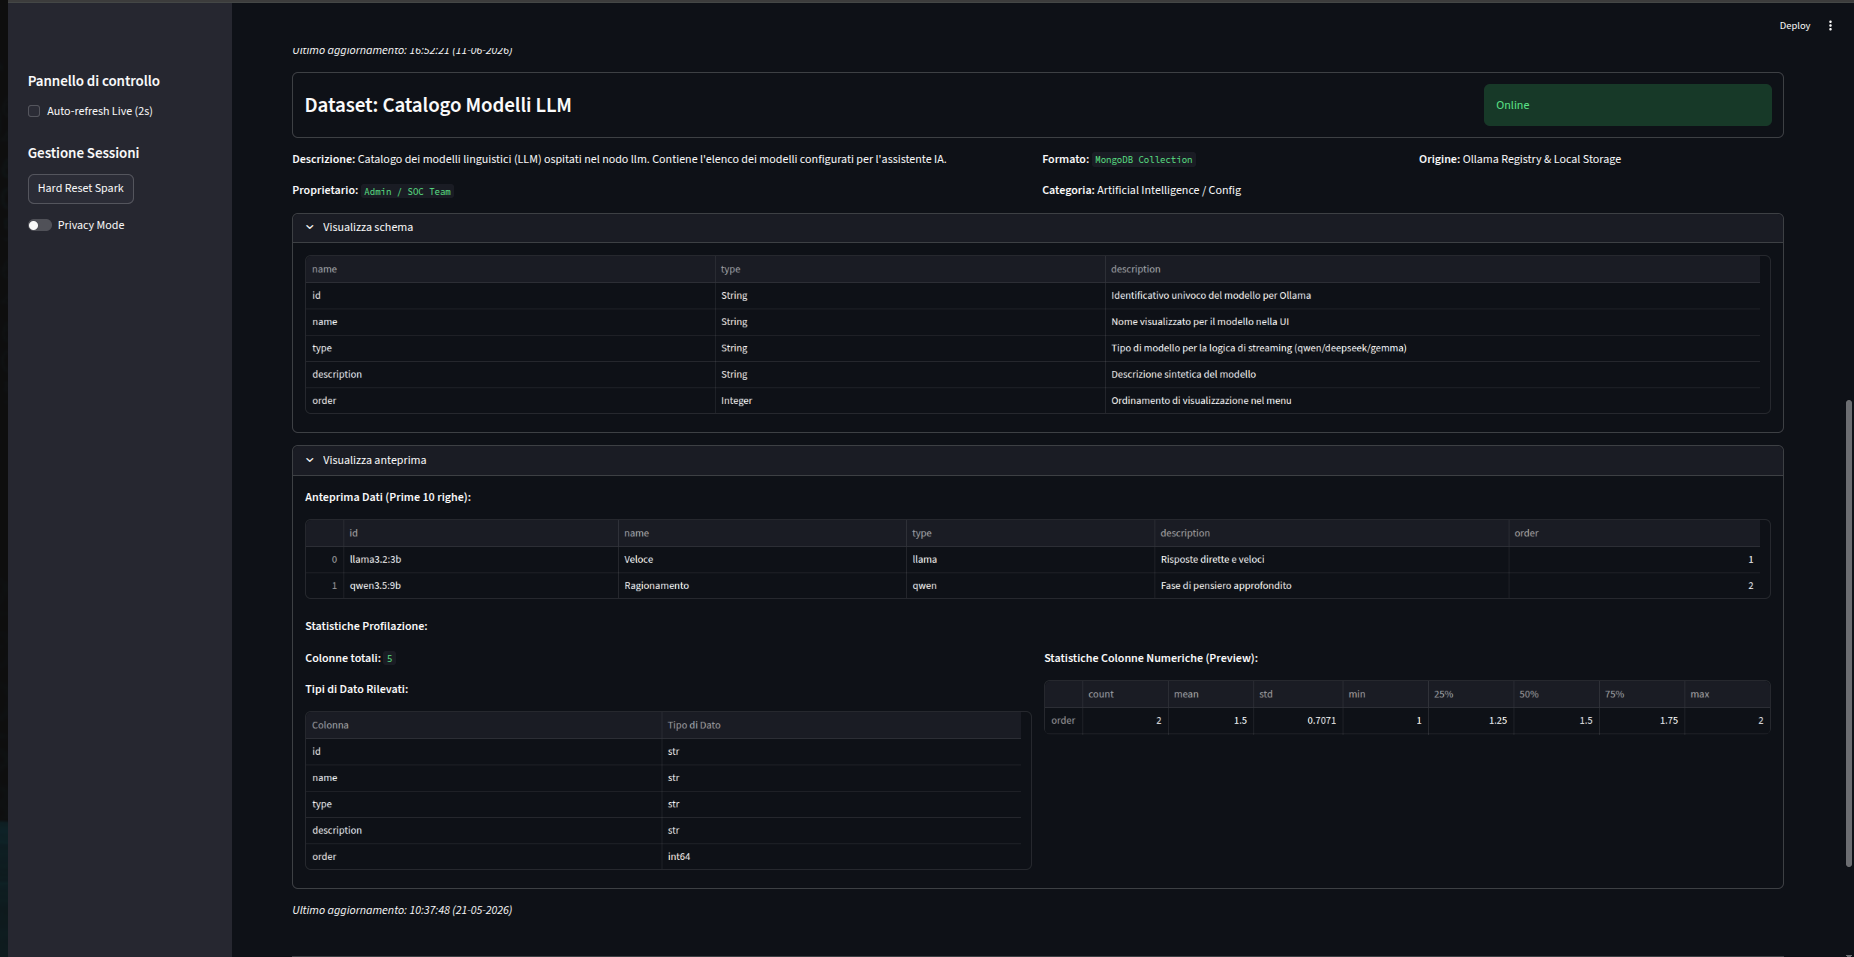
\includegraphics[width=1\textwidth]{figure/catalogo.png}
        \caption{Dashboard che mostra il catalogo degli LLM}
        \label{fig:catalogo}
    \end{figure}
    \subsection{Sniffer}
    Lo sniffer cattura il traffico di rete in tempo reale tramite tcpdump in un ciclo continuo che scrive blocchi di 
    1000 pacchetti, evitando che il file cresca indefinitamente. 
    Un ingestore Python rilegge periodicamente questo file con Scapy, estrae i nuovi pacchetti e li scrive su MongoDB in una capped collection,
     applicando contestualmente le regole di rilevamento/mitigazione descritte in precedenza. Dall'interfaccia 
    è possibile visualizzare gli ultimi pacchetti catturati (con mascheramento opzionale degli IP) e scaricare il 
    file PCAP grezzo per un'analisi approfondita con Wireshark.
    \begin{figure}[H]
        \centering
        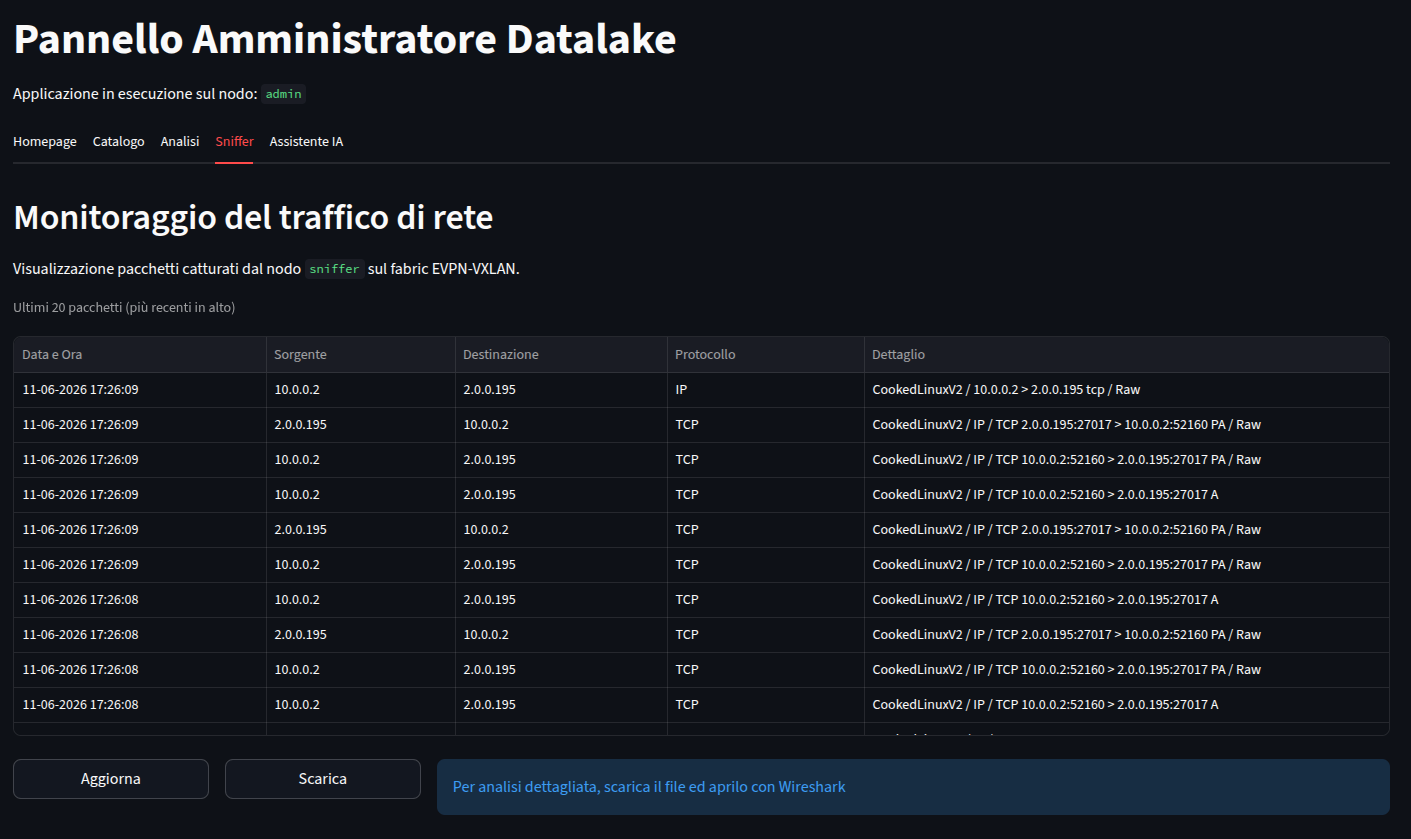
\includegraphics[width=1\textwidth]{figure/sniffer.png}
        \caption{Dashboard che gli ultimi pacchetti catturati dallo sniffer}
        \label{fig:sniffer}
    \end{figure}
    \section{Conclusioni}
    Il progetto ha dimostrato l’applicazione pratica delle principali tecnologie Big Data in uno scenario realistico:
    \begin{itemize}
        \item ingestion eterogenea: dataset storico Parquet (66M+ record) e dati live PCAP, entrambi interrogabili via
                Spark SQL grazie alla Data Federation;
        \item elaborazione distribuita, sfruttando Spark con query SQL complesse su aggregazioni, window functions temporali e join tra sorgenti dati eterogenee;
        \item visualizzazione interattive, che offrono prospettive complementari sul traffico di rete;
        \item MongoDB come Data Lake operazionale (Capped Collection per stream live, Data
                Catalog per i metadati);
        \item integrazione AI: LLM locali con RAG contestuale su dati MongoDB, prompt engineering e generazione automatica di query SQL, senza dipendenza da servizi cloud.
    \end{itemize}
    Link repository: \url{https://github.com/andymacale/primo_progetto_big_data}
\end{document}